\documentclass[10pt,aspectratio=169]{beamer}
% aspectratio can be 1610, 169, 149, 54, 43 and 32
\PassOptionsToPackage{table}{xcolor}
%\usepackage[T1]{fontenc}
\usepackage[utf8]{inputenc}
%\usepackage[T1]{fontenc} % ????
%
\usepackage[french]{babel}
% %\usepackage{emojione}
\usepackage{svg}
\usepackage{wasysym}
%\usepackage{minted}
\usepackage{tabu}

\usepackage{multirow}
\usepackage{multicol}
\usepackage{hyperref}
\usepackage{listings}
\usepackage[table]{xcolor}
\usepackage{amsmath}
\usepackage{amssymb}
\usepackage{xcolor}
\usepackage{pgfplots}
\pgfplotsset{compat=1.17}


\usepackage{circuitikz}
\usepackage{booktabs}

\usepackage{tikz}
\usetikzlibrary{arrows.meta,decorations.pathreplacing,positioning,shapes.arrows}
\usetikzlibrary{babel}

\usepackage{booktabs}
\usepackage{multirow}
\usepackage{array}

\usetheme{Madrid}
\useoutertheme{infolines}

\usepackage[T1]{fontenc}
\usepackage[utf8]{inputenc}
\usepackage{circuitikz}
\usepackage{amsmath}
\usepackage{booktabs}

\lstset{
  language=Ruby,
  basicstyle=\ttfamily\small,
  breaklines=true,
  frame=single,
  showstringspaces=false,
  numbers=left,
  numberstyle=\tiny,
  tabsize=2
}

% Redéfinition du footline pour modifier les proportions
\setbeamertemplate{footline}
{
  \leavevmode%
  \hbox{%
  % Partie gauche (30% de la largeur)
  \begin{beamercolorbox}[wd=0.3\paperwidth,ht=2.25ex,dp=1ex,center]{author in head/foot}%
    \usebeamerfont{author in head/foot}\insertshortauthor
  \end{beamercolorbox}%

  % Partie centrale (40% de la largeur)
  \begin{beamercolorbox}[wd=0.4\paperwidth,ht=2.25ex,dp=1ex,center]{title in head/foot}%
    \usebeamerfont{title in head/foot}\insertshorttitle
  \end{beamercolorbox}%

  % Partie droite (30% de la largeur)
  \begin{beamercolorbox}[wd=0.3\paperwidth,ht=2.25ex,dp=1ex,right]{date in head/foot}%
    \usebeamerfont{date in head/foot}\insertshortdate{}\hspace*{2em}
    \insertframenumber{} / \inserttotalframenumber\hspace*{2ex}
  \end{beamercolorbox}}%
  \vskip0pt%
}



\useinnertheme{circles} % circles, inmargin, rectangles, rounded
\setbeamertemplate{blocks}[default]
\usefonttheme{professionalfonts}

\definecolor{monokaibg}{rgb}{0.153, 0.157, 0.133}
\definecolor{monokaibghl}{rgb}{0.20, 0.20, 0.18}
\definecolor{highlightlbg}{rgb}{0.80, 0.96, 1.00}
\definecolor{lbg}{rgb}{0.96, 0.96, 0.96}
\definecolor{ENSTALBlue}{rgb}{0.1725, 0.3333, 0.4549}
\definecolor{ENSTALCyan}{rgb}{0.3922, 0.7608, 0.7843}
\definecolor{ENSTALYellow}{rgb}{0.9098, 0.8863, 0.2157}
\definecolor{ENSTACMagenta}{rgb}{0.2824, 0.3451, 0.4196}
\definecolor{ENSTACDarkBlue}{rgb}{0.0, 0.3294, 0.4157}
\definecolor{ENSTACBlue}{rgb}{0.0, 0.6353, 0.6627}
\definecolor{ENSTACYellow}{rgb}{0.9804, 0.7137, 0.0}
\definecolor{ENSTACOrange}{rgb}{0.9412, 0.498, 0.2196}
\definecolor{ENSTACRed}{rgb}{0.9294, 0.4196, 0.3804}

\usecolortheme[named=ENSTALBlue]{structure}
%\setbeamercolor{block title}{fg=white,bg=ENSTACDarkBlue}
\setbeamercolor{block title}{fg=white,bg=ENSTALBlue}
\setbeamercolor{block title alerted}{fg=white,bg=ENSTACOrange}
\setbeamercolor{block title example}{fg=white,bg=ENSTALCyan}
\setbeamercolor{alerted text}{fg=ENSTACOrange}
%\setbeamercolor{subtitle}{fg=ENSTALCyan}

%% Remove navigation buttons
\setbeamertemplate{navigation symbols}{}

\setbeamertemplate{itemize item}[circle]            % First level item
\setbeamertemplate{itemize subitem}{\LARGE{-}}       % Second level item
\setbeamertemplate{itemize subitem}{\scriptsize{$\blacktriangleright$}}       % Second level item
%\setbeamertemplate{itemize subitem}{\tiny{$\blacksquare$}}       % Second level item
%\setbeamertemplate{itemize subitem}{\textbf{$\Rightarrow$}}       % Second level item
%\setbeamertemplate{itemize subitem}{\textbf{$\diamond$}}       % Second level item

\definecolor{lightgray}{RGB}{230,230,230}
\definecolor{darkgray}{RGB}{100,100,100}
\definecolor{lila1}{RGB}{183, 132, 183}
\definecolor{lila2}{RGB}{216, 191, 216}
% =================================================
\usepackage{tcolorbox}
\tcbuselibrary{skins}

\newtcolorbox{myblock}[1]{
  colback=lightgray,
  colframe=darkgray,
  coltitle=white,
  title={#1},
  fonttitle=\bfseries,
  boxrule=1pt,
  arc=0pt
}


\newtcolorbox{blockbleu}[1]{
  colframe=lila1,
  colback=lila2,
  coltitle=white,
  title={#1},
  fonttitle=\bfseries,
  boxrule=0pt,
  arc=0pt
}


\titlegraphic{
	%
\includegraphics[height=1.2cm]{images/logo_labsticc.png}\hspace{10em}
	%
\includegraphics[height=0.9cm]{images/logo-ubo.png}\hspace{4em}
	\includegraphics[height=1.2cm]{images/logo_ensta.jpg}
	\hspace{1em}
	%
\includegraphics[height=1.5cm]{images/logo-labsticc.png}
	%\includegraphics[height=1.5cm]{images/logo_ecole_navale.png}
	%\includegraphics[height=1.5cm]{images/logo_imt.jpg}
	%\includegraphics[height=1.5cm]{images/logo_utbm.png}

}

\addtobeamertemplate{frametitle}{}{%
	%% Set ENSTA logo on each frame
	\begin{tikzpicture}[remember picture,overlay]
		\node[anchor=north east,yshift=0.02cm,xshift=-0.05cm] at (current page.north east) {
			\includegraphics[width=2cm]{images/logo_ensta.jpg}
		};
	\end{tikzpicture}
	%% Decrease top margin for the content
	\vspace{-1em}
}




\title{Introduction à l'Electronique Numérique}
%\subtitle{Capture applicative, Architecture et Sécurité}
\author[Jean-Christophe Le Lann]{
	Jean-Christophe Le Lann\\
	\vspace{0.75em}
	%\footnotesize{\texttt{jean-christophe.le\_lann@ensta.fr}}
  \footnotesize{Cours 1A}
}
%\institute{ENSTA Bretagne}
%\date{18 Juillet 2025}
%\date{\today}


% \AtBeginSection[]
% {
% 	\begin{frame}
% 		\frametitle{Plan de la présentation}
% 		\tableofcontents[currentsection]
% 	\end{frame}
% }

\AtBeginSection[]{
  \begin{frame}
  \vfill
  \centering
  \begin{beamercolorbox}[sep=8pt,center,shadow=true,rounded=true]{title}
			\usebeamerfont{title}~\insertsectionnumber -- ~\insertsectionhead\par%
  \end{beamercolorbox}
  \vfill
  \end{frame}
}

\newcommand<>{\insertExampleCode}[2][0]{
	\begin{onlyenv}#3
		\inputminted[bgcolor=lbg,fontsize=\footnotesize,highlightcolor=highlightlbg,highlightlines={#1}]{asm}{#2}
	\end{onlyenv}
}

\newtcolorbox{ideabox}{
    colback=blue!5!white, % Fond bleu clair
    colframe=blue!75!black, % Bordure bleue
    title={Idée}, % Titre avec icône (FontAwesome)
    fonttitle=\bfseries,
    enhanced, % Améliorations graphiques
    attach boxed title to top left={xshift=5mm, yshift=-2mm},
    boxed title style={colback=blue!75!black, colframe=blue!75!black}
}

\newcommand{\triangalert}[1]{\alert{\textcolor{blue}{$\triangleright$} #1}}

\newcommand{\orangetriangalert}[1]{%
    {\color{orange}\textbf{$\blacktriangleright$} #1}%
}
%===============================xxx================================================================================
\begin{document}

%\frame{\titlepage}

\begin{frame}
  \titlepage
	% \begin{block}{\centering \large Capture applicative, Architecture et Sécurité}
	% \end{block}
\end{frame}

% \begin{frame}{De l'idée au circuit}
%     \begin{columns}[c]  % [T] aligne en haut, [c] centré, [b] en bas
%         \begin{column}{0.4\textwidth}  % Colonne de gauche (50% de la largeur)
%           \begin{enumerate}
%
%             \item \textbf{Abstraction technologique} :
%             \begin{itemize}
%               \item Nouveaux modes de pensée
%               \item Approche \textbf{constructive} et \textbf{scalable}
%             \end{itemize}
%
%             \item \textbf{Double discrétisation} :
%             \begin{itemize}
%               \item discrétisation des \textbf{valeurs}
%               \item discrétisation du \textbf{temps}
%             \end{itemize}
%
%             \item \textbf{Evitement des fluctuations physiques} :
%             \begin{itemize}
%               \item Indépendance vis-à-vis de la température.
%               \item Indépendance vis-à-vis des courants, tensions, etc.
%             \end{itemize}
%
%           \end{enumerate}
%         \end{column}
%
%         \begin{column}{0.6\textwidth}  % Colonne de droite (50% de la largeur)
%             \centering
%             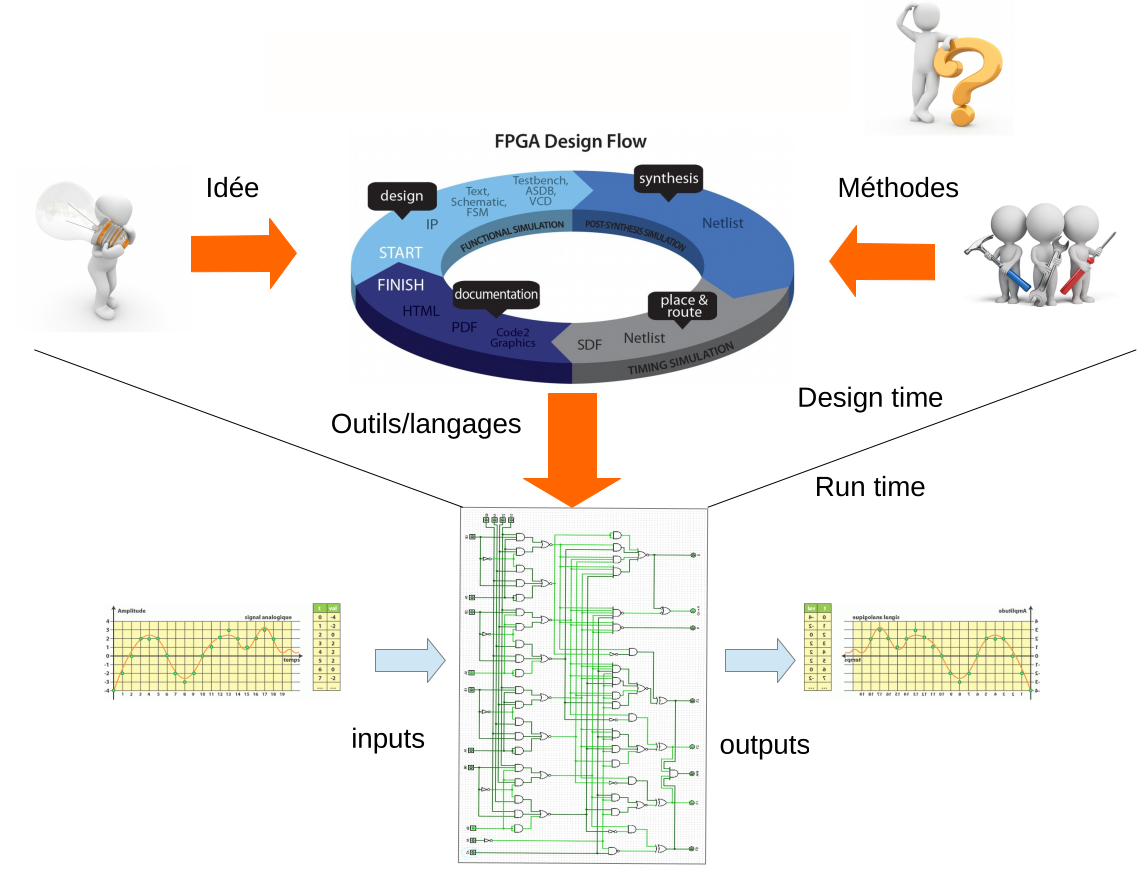
\includegraphics[scale=0.3]{./images/idee_circuit.png}
%         \end{column}
%     \end{columns}
% \end{frame}

%========================================================================================
\begin{frame}{De l'idée au circuit}
  \begin{center}
    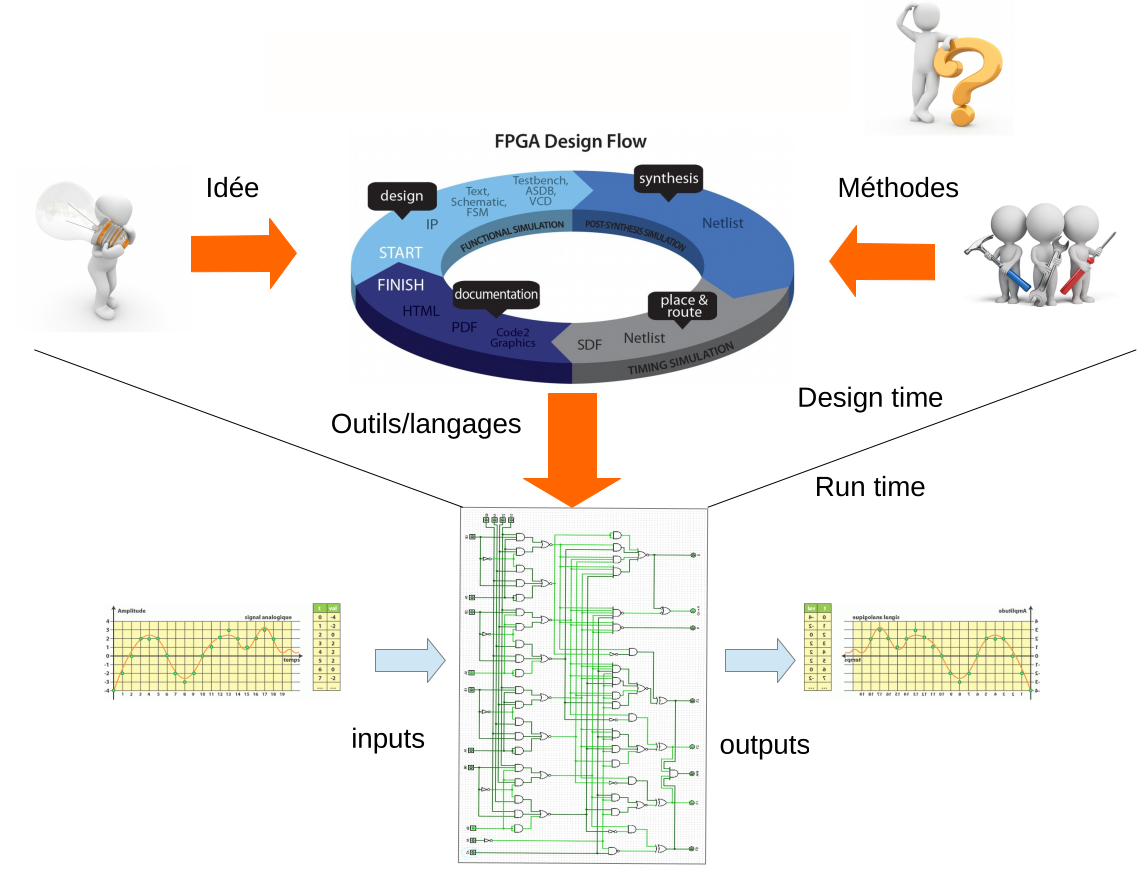
\includegraphics[scale=0.32]{./images/idee_circuit.png}
  \end{center}
\end{frame}

\begin{frame}{Numérisation}
  \begin{center}
    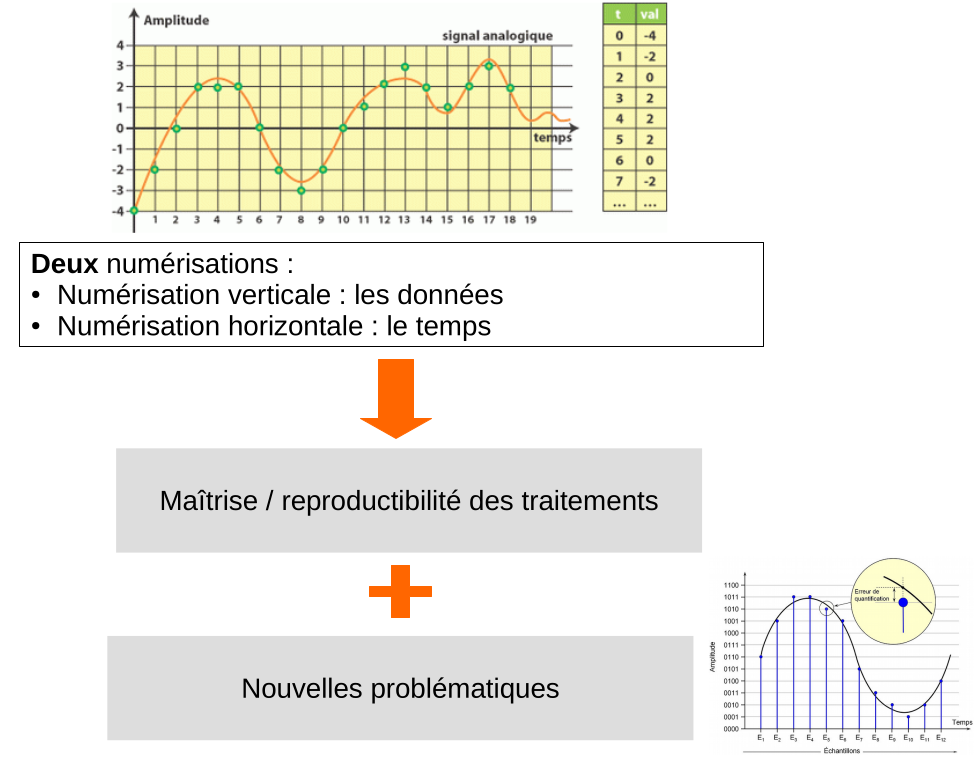
\includegraphics[scale=0.25]{./images/numerisation.png}
  \end{center}
\end{frame}
%========================================================================================
\begin{frame}{Plan}
  \tableofcontents
\end{frame}

\begin{frame}{Objectifs}
  \begin{columns}
    \begin{column}{0.5\textwidth}
      \begin{enumerate}
        \item Comprendre les fondements de la conception des systèmes numériques :
        \begin{itemize}
          \item Logique booléenne : combinatoire et séquentielle.
          \item Calcul sur silicium, chemin de données
          \item Machines d'états finis : contrôleurs / automates
          \item Principe des Micro-architectures
          \item Initiation à VHDL au niveau logique et structurel
        \end{itemize}

        \item Premiers pas vers les systèmes embarqués :
        \begin{itemize}
          \item Processeurs, périphériques, communication
        \end{itemize}
      \end{enumerate}
    \end{column}

    \begin{column}{0.5\textwidth}
      \begin{center}
        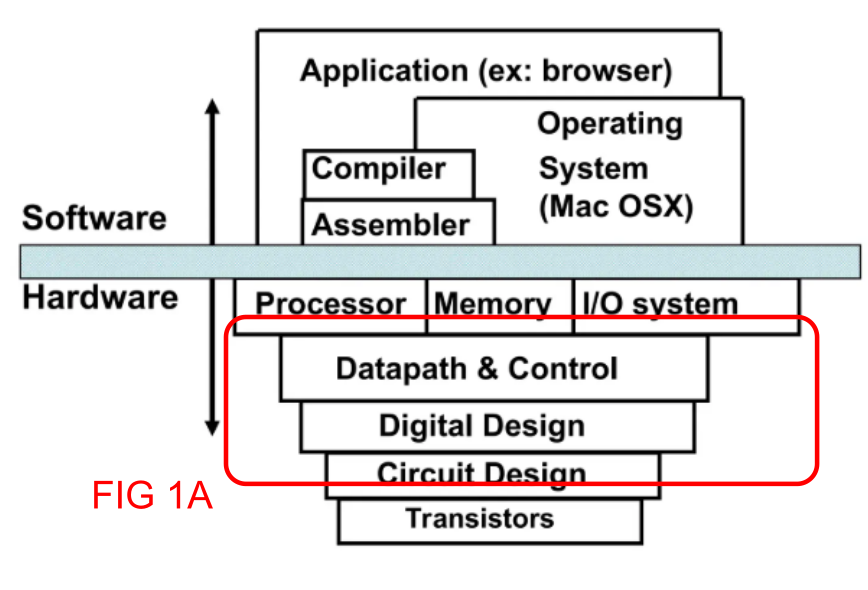
\includegraphics[scale=0.25]{./images/scope.png}
      \end{center}
    \end{column}
  \end{columns}


\end{frame}

%========================================================================================
\section{Physique des semi-conducteurs et micro-électronique : un aperçu}
%========================================================================================
\begin{frame}{Le Silicium : élément chimique}
  \begin{center}
    %\includesvg[scale=0.35]{images/silicium_atome}
    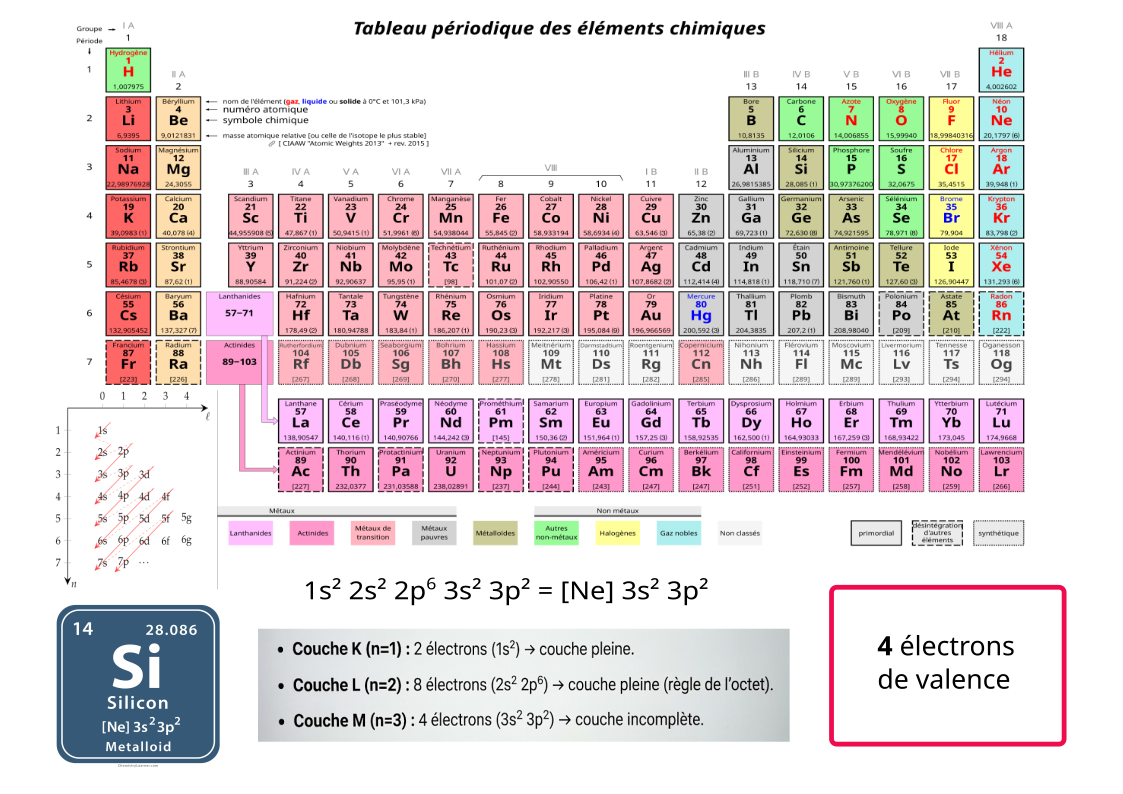
\includegraphics[scale=0.35]{images/silicium_atome.png}
  \end{center}
\end{frame}

\begin{frame}{Le Silicium : à partir de la Silice}
 \begin{enumerate}

   \item \textbf{Extraction} : réduction carbothermique de la silice
   \begin{itemize}
     \item Réaction chimique à 3000° : SiO2 + 2C → Si (liquide) + 2CO (gaz)
     \item Source de carbone : charbon, coke,...
     \item Pureté 98-99.5 \% insuffisante pour l'Electronique (silicium métallurgique MG-Si)
   \end{itemize}

   \item \textbf{Purification} : Procédé \textbf{Siemens}
   \begin{itemize}
     \item Hydrochloration du silicium métallurgique : trichlorosilane $SiHCl_3$ (gazeux)
     \item Si + 3 HCl → SiHCl3 + H2
     \item Distillation : chauffage à 1100°. Décomposition et obtention de "germes".
     \item Pureté 99.9999999\% (polycristallin) voire plus pour l'Electronique.
   \end{itemize}

   \item \textbf{Obtention d'un monocristal} : Procédé \textbf{Czokralski}
   \begin{itemize}
     \item Fusion et germination.
     \item Tirage et rotation.
     \item Formation du lingot.
   \end{itemize}

 \end{enumerate}
\end{frame}

\begin{frame}{Le Silicium : méthode Czokralski}
  \begin{center}
    \includesvg[scale=0.4]{images/silicium_czokralski}
  \end{center}
\end{frame}

\begin{frame}{Le Silicium : cristallogaphie}
  \begin{center}
    %\includesvg[scale=0.35]{images/silicium_cristal}
    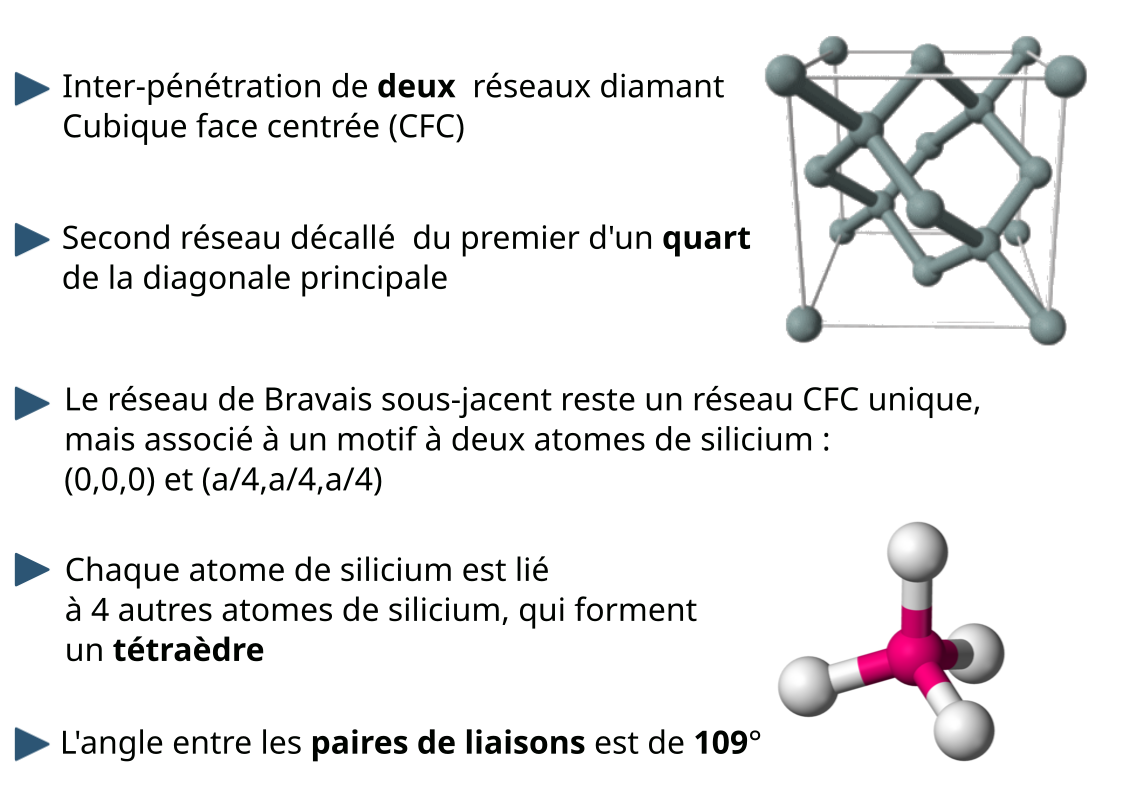
\includegraphics[scale=0.35]{images/silicium_cristal.png}
  \end{center}
\end{frame}

\begin{frame}{Le Silicium : cristallogaphie}
  \begin{center}
    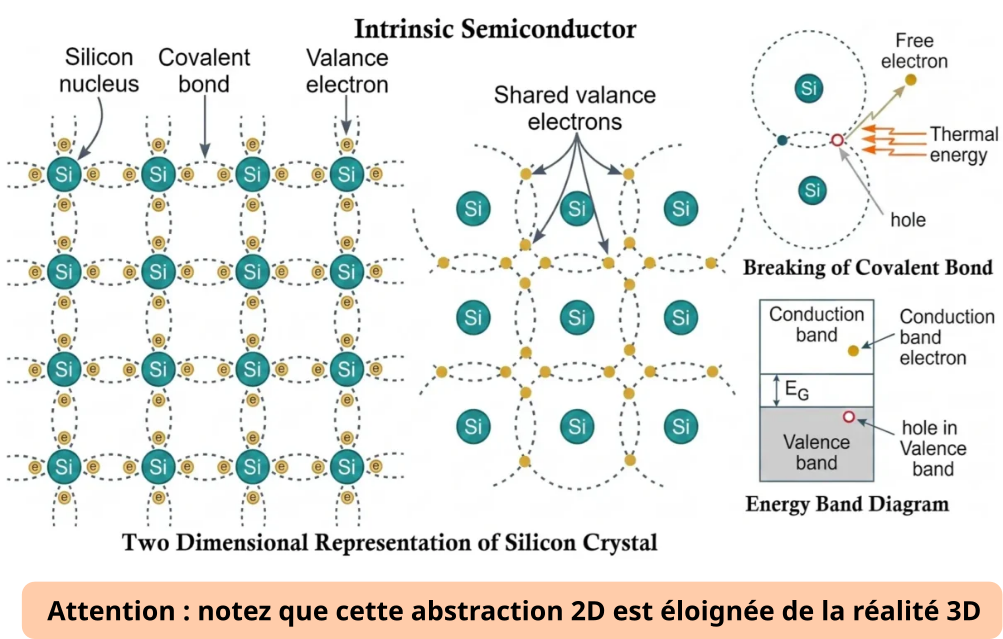
\includegraphics[scale=0.4]{images/silicium_thermal_energy.png}
  \end{center}
\end{frame}

\begin{frame}{Le Silicium : théorie des bandes}
  \begin{center}
    \includesvg[scale=0.38]{images/silicium_bandes.svg}
  \end{center}
\end{frame}

\begin{frame}{Le Silicium : dopage N et P}
  \begin{center}
    \includesvg[scale=0.35]{images/silicium_bore_antimoine.svg}
    %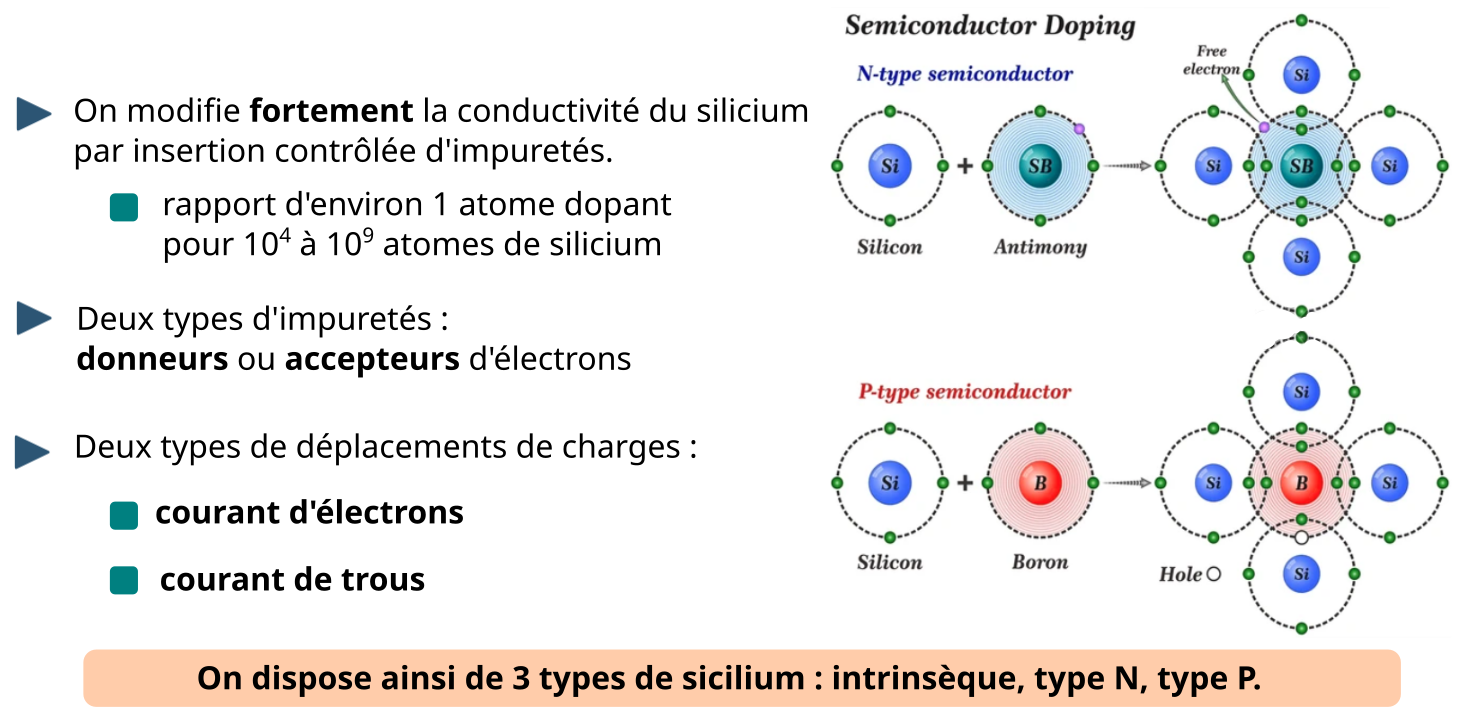
\includegraphics[scale=0.4]{images/silicium_bore_antimoine.png}
  \end{center}
\end{frame}

\begin{frame}{Jonction P-N : mise en contact de deux types de silicium }

\begin{enumerate}
  \item Mise en contact et diffusion
  \begin{itemize}
    \item \textbf{Loi de Fick} : les porteurs majoritaires diffusent.
    \item Les électrons de N vers P, les trous de P vers N
    \item \textbf{Recombinaisons} au voisinage immédiat de l'interface.
  \end{itemize}
  \item La \textbf{zone de déplétion} (ZCE) : zone vidée de ses porteurs libres
  \begin{itemize}
    \item côté N : des ions donneurs positifs non compensés
    \item côté P : des ions accepteurs négatifs non compensés
    \item ZCE : région dépourvue de porteurs mobiles mais chargée électriquement.
  \end{itemize}

  \item \textbf{Champ interne} et barrière de potentiel
  \begin{itemize}
    \item un champ électrique interne $\vec{E}$, orienté de N vers P, qui s'oppose à la diffusion.
  \end{itemize}

  \item Équilibre dynamique :
  \begin{itemize}
    \item Une barrière de potentiel $V_0$ s'établit (environ 0,7 V pour le silicium).
    \item Le courant de diffusion (dû au gradient) équilibre exactement le courant de conduction (dû  au champ électrique).
    \item Le niveau de Fermi $E_F$ devient continu à travers tout le matériau.
  \end{itemize}
\end{enumerate}
\end{frame}

%\begin{frame}{Jonction P-N : polarisation }
%
% \begin{enumerate}
%   \item Polarisation directe
%   \begin{itemize}
%     \item + côté P, - côté N.
%     \begin{itemize}
%       \item La tension externe s'oppose au champ interne :
%       \item la barrière de potentiel diminue. la ZCE se rétrécit
%       \item la diffusion des majoritaires redevient dominante
%       \item le courant croît exponentiellement avec V.
%     \end{itemize}
%     \item Loi de Shockley : $I = I_0(e^{V/V_T} - 1)$
%   \end{itemize}
%   \item Polarisation inverse
%   \begin{itemize}
%     \item champ externe renforce le champ interne
%     \item la ZCE s'élargit
%     \item très faible courant
%   \end{itemize}
% \end{enumerate}
% \end{frame}

\begin{frame}{Jonction P-N : polarisation}
    \begin{columns}[T]  % [T] aligne en haut, [c] centré, [b] en bas
        \begin{column}{0.5\textwidth}  % Colonne de gauche (50% de la largeur)
          \begin{enumerate}
            \item Polarisation directe
            \begin{itemize}
              \item + côté P, - côté N.
              \begin{itemize}
                \item La tension externe s'oppose au champ interne.
                \item la barrière de potentiel diminue. la ZCE se rétrécit.
                \item la diffusion des majoritaires redevient dominante.
                \item le courant croît exponentiellement avec V.
              \end{itemize}
              \item Loi de Shockley : $I = I_0(e^{V/V_T} - 1)$
            \end{itemize}
            \item Polarisation inverse
            \begin{itemize}
              \item champ externe renforce le champ interne
              \item la ZCE s'élargit
              \item très faible courant
            \end{itemize}
          \end{enumerate}
        \end{column}

        \begin{column}{0.5\textwidth}  % Colonne de droite (50% de la largeur)
            \centering
            \includesvg[width=\textwidth, height=0.7\textheight, keepaspectratio]{./images/jonction_1}
            % ou avec des dimensions fixes :
            % \includesvg[width=5cm, height=5cm]{chemin/vers/votre_fichier}
        \end{column}
    \end{columns}
\end{frame}

\begin{frame}{Transistor bipolaire : structure}
  \begin{columns}[T]  % [T] aligne en haut, [c] centré, [b] en bas
        \begin{column}{0.45\textwidth}  % Colonne de gauche (50% de la largeur)
          \begin{itemize}
            \item Deux jonctions PN dos-à-dos : type NPN ou PNP
            \item Trois régions : émetteur, base, collecteur
            \item Base fine et faiblement dopée
            \item Jonction émetteur-base polarisée en direct
            \item Jonction base-collecteur polarisée en inverse
            \item Effet transistor : le courant de base contrôle le courant de collecteur
          \end{itemize}
        \end{column}

        \begin{column}{0.55\textwidth}  % Colonne de droite (50% de la largeur)
            \centering
            \includegraphics[scale=0.18]{./images/bipolar.jpg}
        \end{column}
    \end{columns}
\end{frame}

\begin{frame}{Transistor bipolaire : fonctionnement}
\begin{itemize}
    \item Gain en courant $\beta = I_C / I_B$ (typiquement 50 à 300)
    \item Régime actif : amplification (usage analogique)
    \item Régime saturé : interrupteur fermé (les 2 jonctions en direct)
    \item Régime bloqué : interrupteur ouvert (les 2 jonctions en inverse)
    \item Relation fondamentale : $I_E = I_B + I_C$
    \item Applications : amplification, commutation, logique TTL
\end{itemize}
\end{frame}
%
% \begin{frame}{Transistor bipolaire : fonctionnement}
%   \begin{itemize}
%   \item  \textbf{Injection} : La polarisation en direct de la jonction EB "pousse" les trous (porteurs majoritaires de l'émetteur P) à travers la jonction pour les injecter dans la base N.
%   \item \textbf{Traversée de la base} : Comme la base est très fine et faiblement dopée, la grande majorité des trous injectés ne trouvent pas d'électrons avec lesquels se recombiner. Ils diffusent donc à travers la base jusqu'à la jonction CB.
%   \item \textbf{Collecte} : La jonction CB étant polarisée en inverse, elle crée un champ électrique intense dans sa zone de déplétion. Ce champ "aspire" immédiatement les trous qui arrivent de la base et les accélère vers le collecteur P.
%   \item \textbf{Recombinaison} (Courant de base) : Une très petite fraction des trous (typiquement 1 \% à 5 \%) se recombine avec les électrons dans la base. Pour maintenir la neutralité électrique, le circuit de base doit fournir continuellement de nouveaux électrons, ce qui constitue le faible courant de base.
%   \end{itemize}
% \end{frame}

\begin{frame}{Transistors MOS (nmos)}
  \begin{columns}[c] % [T] aligne en haut, [c] centré, [b] en bas
    \begin{column}{0.5\textwidth}  % Colonne de gauche (50% de la largeur)
      \begin{itemize}
        \item Transistor à \textbf{effet de champ} (FET) à canal N, constitué d’un substrat P, de deux zones N+ (Source et Drain) et d’une grille isolée par un oxyde ($SiO_2$).
        \item Commande \textbf{par la tension} grille-source $V_{GS}$
        \item Création un canal conducteur (ou non) d’électrons entre Source et Drain.
        \item Inconvénient : un inverseur NMOS utilise une résistance de pull-up.
      \end{itemize}
    \end{column}

    \begin{column}{0.5\textwidth}  % Colonne de droite (50% de la largeur)
        \begin{center}
          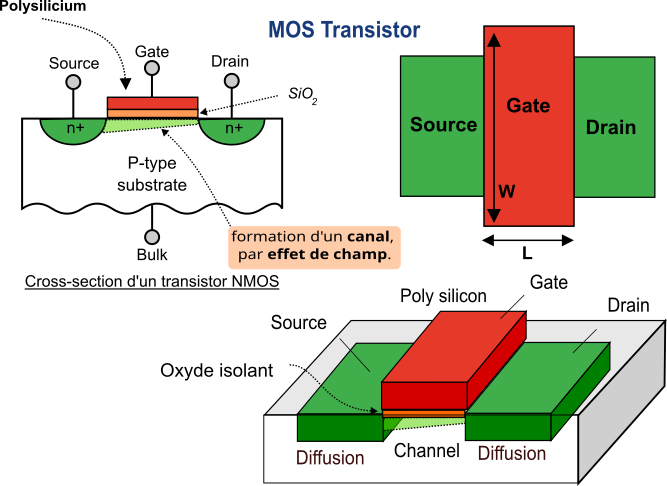
\includegraphics[scale=0.43]{./images/nmos_diagram.png}
        \end{center}
    \end{column}
    \end{columns}
\end{frame}



%===================================================

\begin{frame}{Le procédé de photolithographie}

\begin{columns}[T,onlytextwidth]

  % ---- Colonne de gauche : points clés ----
  \begin{column}{0.47\textwidth}
    \footnotesize
    \begin{itemize}\setlength{\itemsep}{3pt}
      \item \textbf{Principe} : transférer un motif géométrique d'un masque vers une résine photosensible déposée sur une plaquette (\emph{wafer})
      \item \textbf{Dépôt} : enduction centrifuge (\emph{spin coating}) d'un film uniforme
      \item \textbf{Insolation} : exposition UV à travers un masque optique portant le motif
      \item \textbf{Développement} : dissolution sélective des zones exposées (résine positive) ou non exposées (négative)
      \item \textbf{Gravure} : transfert du motif dans le substrat (voie humide ou plasma)
      \item \textbf{Retrait} de la résine (\emph{stripping})
      \item Résolution limitée par la diffraction $\Rightarrow$ UV profond, immersion, EUV
    \end{itemize}
  \end{column}

  % ---- Colonne de droite : schéma ----
  \begin{column}{0.51\textwidth}
    \centering
    \includegraphics[width=\textwidth]{./images/photolitho_v2.pdf}
  \end{column}

\end{columns}

\end{frame}


\begin{frame}{ASML : le leader de la photo-lithographie}
  \begin{columns}
    \begin{column}{0.7\textwidth}
      \begin{center}
        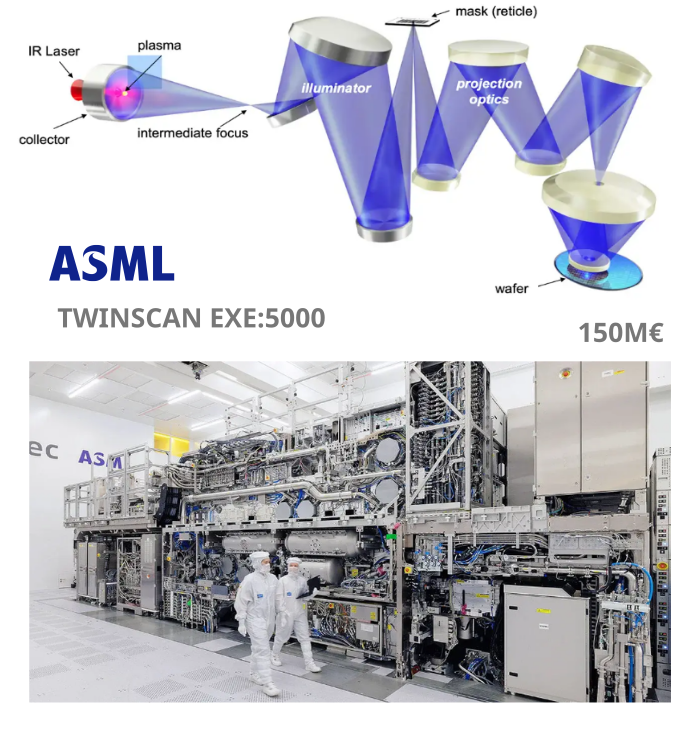
\includegraphics[scale=0.37]{./images/asml.png}
      \end{center}
    \end{column}
    \begin{column}{0.3\textwidth}
      \begin{center}
        \includegraphics[scale=0.4]{./images/ic_3d.jpg}
      \end{center}
    \end{column}
  \end{columns}
\end{frame}

\section{Technologie CMOS : Complementary Metal Oxyde Semiconductor}

\begin{frame}{CMOS --- Transistors CMOS }
  \begin{columns}
    \begin{column}{0.5\textwidth}  % Colonne de droite (50% de la largeur)
      \begin{alertblock}{Paradigme dominant}
        Fondement de la microélectronique numérique actuelle
      \end{alertblock}
      \begin{itemize}
        \item Association de transistors \textbf{NMOS} et \textbf{PMOS} sur un même substrat.
        \item NMOS : conduit lorsque la grille est à $V_{DD}$
        \item PMOS : conduit lorsque la grille est à $0\,$V
        \begin{itemize}
          \item Se substitue à la résistance de pull-up du NMOS.
          \item Montage \textbf{dual} : série $\rightleftarrows$ parallèle.
        \end{itemize}
        \item Effet de champ : la \textbf{tension} de grille contrôle le canal.
        \item Isolation par \textbf{oxyde de grille} $\Rightarrow$ haute impédance d'entrée.
      \end{itemize}
    \end{column}

    \begin{column}{0.5\textwidth}  % Colonne de droite (50% de la largeur)
        \begin{center}
          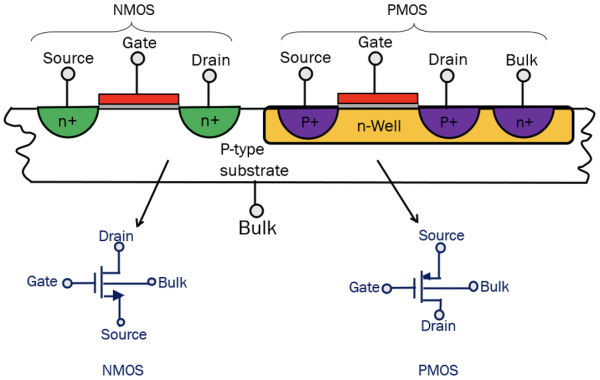
\includegraphics[scale=0.45]{./images/cmos_0.png}
        \end{center}
    \end{column}
  \end{columns}
\end{frame}

\begin{frame}{Le modèle de Schichman--Hodges : caractéristiques $I_D(V_{DS})$}

\begin{alertblock}{Physique}
 Caractérisation du comportement \textit{analogique} du MOS.
\end{alertblock}

\begin{columns}[T,totalwidth=\textwidth]

% ---------- Colonne de gauche : équations ----------
\begin{column}{0.48\textwidth}

\footnotesize
\textbf{1. Blocage} \quad ($V_{GS} - V_T \leq 0$)
\[
I_D = 0
\]

\vspace{1mm}
\textbf{2. Zone linéaire} \quad ($0 < V_{DS} < V_{GS}-V_T$)
\[
I_D = k_n \tfrac{W}{L}\!\left[(V_{GS}\!-\!V_T)V_{DS} - \tfrac{V_{DS}^2}{2}\right]\!\left(1+\lambda V_{DS}\right)
\]

\vspace{1mm}
\textbf{3. Saturation} \quad ($V_{DS} \geq V_{GS}-V_T$)
\[
I_D = \frac{k_n}{2} \frac{W}{L}(V_{GS}-V_T)^2\left(1+\lambda V_{DS}\right)
\]

\vspace{2mm}
\scriptsize
$k_n=\mu_n C_{ox}$ (transconductance) $\;\cdot\;$ $V_T$ (seuil) $\;\cdot\;$ $\lambda$ (modulation de canal) $\;\cdot\;$ $W/L$ (géométrie)

\vspace{2mm}
\footnotesize
\alert{Un seul jeu d'équations décrit tout le comportement}, du blocage à la saturation.

\end{column}

% ---------- Colonne de droite : courbes caractéristiques ----------
\begin{column}{0.52\textwidth}
  \begin{center}
    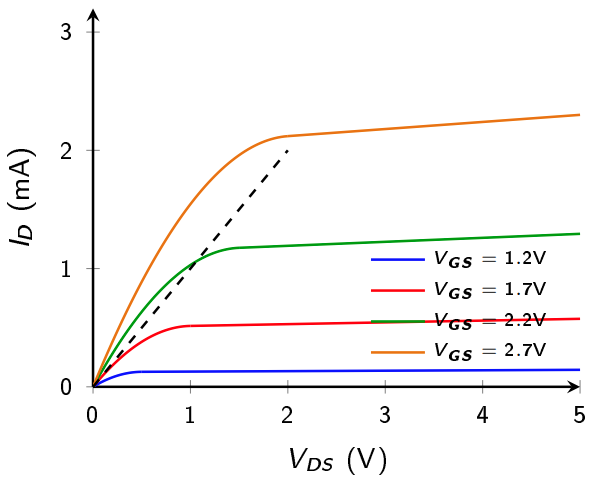
\includegraphics[scale=0.3]{./images/caract_mos.png}
  \end{center}
\end{column}

\end{columns}

\end{frame}

\begin{frame}{Le transistor comme interrupteur commandé}
  \begin{columns}
    \begin{column}{0.5\textwidth}
      \textbf{Transistor NMOS}
      \begin{itemize}
        \item Conduit (interrupteur fermé) si \textbf{Grille = 1}
        \item Bloqué si Grille = 0
        \item \fbox{Transmet bien un \textbf{0} logique}
      \end{itemize}
      \vspace{0.5cm}
      \textbf{Transistor PMOS}
      \begin{itemize}
        \item Conduit (interrupteur fermé) si \textbf{Grille = 0}
        \item Bloqué si Grille = 1
        \item \fbox{Transmet bien un \textbf{1} logique}
      \end{itemize}
    \end{column}
    \begin{column}{0.5\textwidth}
      \centering
      \begin{circuitikz}[scale=1.0]
        \draw (0,0) node[nmos, anchor=D](M1){};
        \draw (M1.G) node[left=0.3cm]{$G$};
        \draw (M1.S) node[below=0.2cm]{$S$};
        \draw (M1.D) node[above=0.2cm]{$D$};
      \end{circuitikz}
      \hspace{0.5cm}
      \begin{circuitikz}[scale=1.0]
        \draw (0,0) node[pmos, anchor=D](M2){};
        \draw (M2.G) node[left=0.3cm]{$G$};
        \draw (M2.S) node[above=0.2cm]{$S$};
        \draw (M2.D) node[below=0.2cm]{$D$};
      \end{circuitikz}
    \end{column}
  \end{columns}
\end{frame}
%
\begin{frame}{Table de fonctionnement simplifiée}
  \centering
  \begin{tabular}{ccc}
    \toprule
    Entrée grille & NMOS & PMOS \\
    \midrule
    0 & bloqué & passant \\
    1 & passant & bloqué \\
    \bottomrule
  \end{tabular}
  \vspace{0.5cm}

  \begin{block}{Idée fondatrice du CMOS}
    On associe systématiquement un réseau de NMOS (relié à la masse)
    et un réseau de PMOS \emph{dual} (relié à l'alimentation $V_{DD}$)
    pour qu'à chaque instant \textbf{un seul} des deux réseaux conduise.
  \end{block}
\end{frame}
%
% ------------------------------------------------------------
%\section{L'inverseur CMOS}

\begin{frame}{L'inverseur CMOS : la porte de base}
  \begin{columns}
    \begin{column}{0.35\textwidth}
      \begin{circuitikz}[scale=1.1, transform shape]
        % --- Alimentation ---
        \draw (0,4.6) node[above]{$V_{DD}$};
        \draw (0,4.6) to[short] (0,4.1);
        % --- PMOS ---
        \draw (0,4.1) node[pmos, anchor=S](P1){};
        % --- Noeud de sortie Y ---
        \draw (P1.D) to[short] (0,2.6);
        \draw (0,2.6) to[short] (0.7,2.6) node[right]{$Y$};
        % --- NMOS ---
        \draw (0,2.6) node[nmos, anchor=D](N1){};
        % --- Connexion des grilles ---
        \draw (P1.G) -- ++(-0.8,0) coordinate(pgate);
        \draw (N1.G) -- ++(-0.8,0) coordinate(ngate);
        \draw (pgate) -- (ngate);
        % --- Entrée A alignée avec Y ---
        \coordinate (aPoint) at (pgate |- N1.D);
        \draw (aPoint) -- ++(-0.5,0) node[left]{$A$};
        % --- Masse ---
        \draw (N1.S) to[short] (0,1.1);
        \draw (0,1.1) node[ground]{};
      \end{circuitikz}
    \end{column}
    \begin{column}{0.65\textwidth}
      \begin{itemize}
        \item Entrée $A$ commune aux deux grilles
        \item PMOS en haut (côté $V_{DD}$)
        \item NMOS en bas (côté masse)
        \item Si $A=0$ : PMOS passant, NMOS bloqué $\Rightarrow Y=1$
        \item Si $A=1$ : PMOS bloqué, NMOS passant $\Rightarrow Y=0$
      \end{itemize}
      \vspace{0.3cm}
      \[ Y = \overline{A} \]
    \end{column}
  \end{columns}
\end{frame}

\begin{frame}{L'inverseur CMOS : chronogramme}
  \begin{center}
    %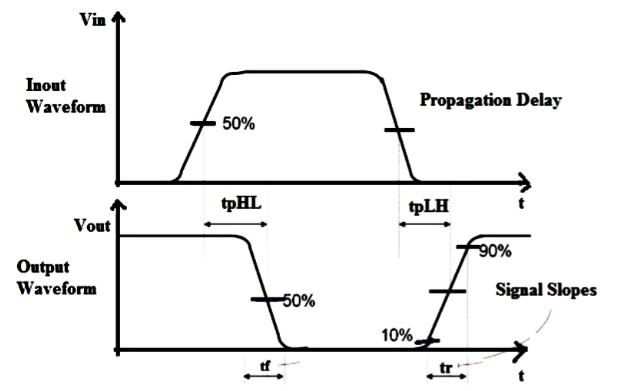
\includegraphics[scale=0.5]{./images/inverter_slopes.png}
    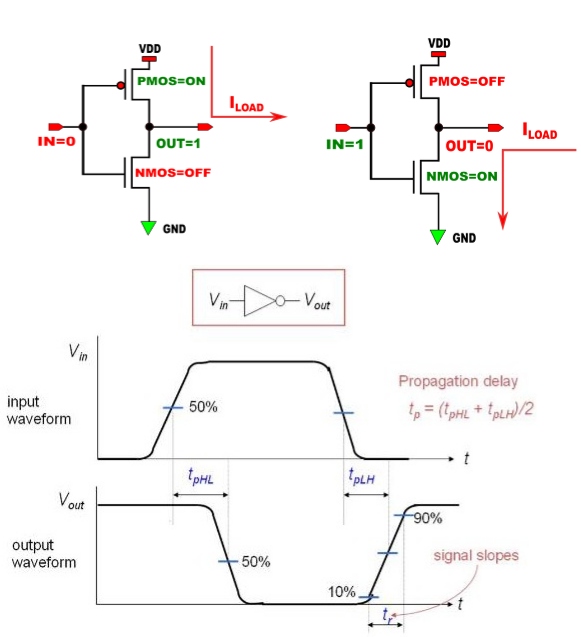
\includegraphics[scale=0.45]{./images/inverter.png}
  \end{center}
\end{frame}

\begin{frame}{Porte NAND à 2 entrées : montage dual}
  \begin{columns}
    \begin{column}{0.35\textwidth}
      \begin{circuitikz}[scale=1.0, transform shape]
        % --- Rail VDD ---
        \draw (-1.6,6.0) node[above]{$V_{DD}$} to[short] (2.2,6.0);

        % --- PMOS A (gauche) ---
        \draw (-0.8,6.0) to[short] (-0.8,5.6);
        \node[pmos, anchor=S] (Pa) at (-0.8,5.6) {};
        \draw (Pa.G) -- ++(-0.3,0) node[left]{$A$};

        % --- PMOS B (droite) ---
        \draw (1.4,6.0) to[short] (1.4,5.6);
        \node[pmos, anchor=S] (Pb) at (1.4,5.6) {};
        \draw (Pb.G) -- ++(-0.3,0) node[left]{$B$};

        % --- Jonction des deux drains PMOS (en parallele) ---
        \draw (Pa.D) -- (-0.8,4.3) -- (0.3,4.3);
        \draw (Pb.D) -- (1.4,4.3) -- (0.3,4.3);
        \draw (0.3,4.3) -- (0.3,3.6);

        % --- Noeud de sortie Y, sorti sur le cote pour eviter le chevauchement ---
        \draw (0.3,3.6) to[short] (1.6,3.6) node[right]{$Y$};
        \filldraw (0.3,3.6) circle (0.05);

        % --- NMOS A (haut de la pile) ---
        \node[nmos, anchor=D] (Na) at (0.3,3.6) {};
        \draw (Na.G) -- ++(-0.9,0) node[left]{$A$};

        % --- NMOS B (bas de la pile), en serie avec Na ---
        \node[nmos, anchor=D] (Nb) at (0.3,2.3) {};
        \draw (Na.S) -- (Nb.D);
        \draw (Nb.G) -- ++(-0.9,0) node[left]{$B$};

        % --- Masse ---
        \draw (Nb.S) -- (0.3,1.0) node[ground]{};
      \end{circuitikz}
    \end{column}
    \begin{column}{0.65\textwidth}
      \begin{itemize}
        \item NMOS $A$ et $B$ en \textbf{série} $\to$ conduit
          seulement si $A=1$ ET $B=1$
        \item PMOS $A$ et $B$ en \textbf{parallèle} (dual)
        \item $Y=0$ uniquement si $A=B=1$
      \end{itemize}
      \[ Y = \overline{A \cdot B} \]
    \end{column}
  \end{columns}
\end{frame}

\begin{frame}{Pourquoi ça marche : jamais de court-circuit}
  \begin{itemize}
    \item En régime statique, un seul chemin conducteur existe entre
      $V_{DD}$ et $Y$, ou entre $Y$ et la masse — jamais les deux.
    \item Conséquence : \textbf{pas de consommation statique}
      (hors fuites), contrairement aux logiques NMOS seules
      (résistance de charge) ou bipolaires.
    \item La consommation du CMOS est essentiellement
      \textbf{dynamique} : elle a lieu lors des commutations
      (charge/décharge des capacités de sortie).
  \end{itemize}
\end{frame}

\begin{frame}{Dualité N-P en CMOS : autre exemple}
  \begin{center}
    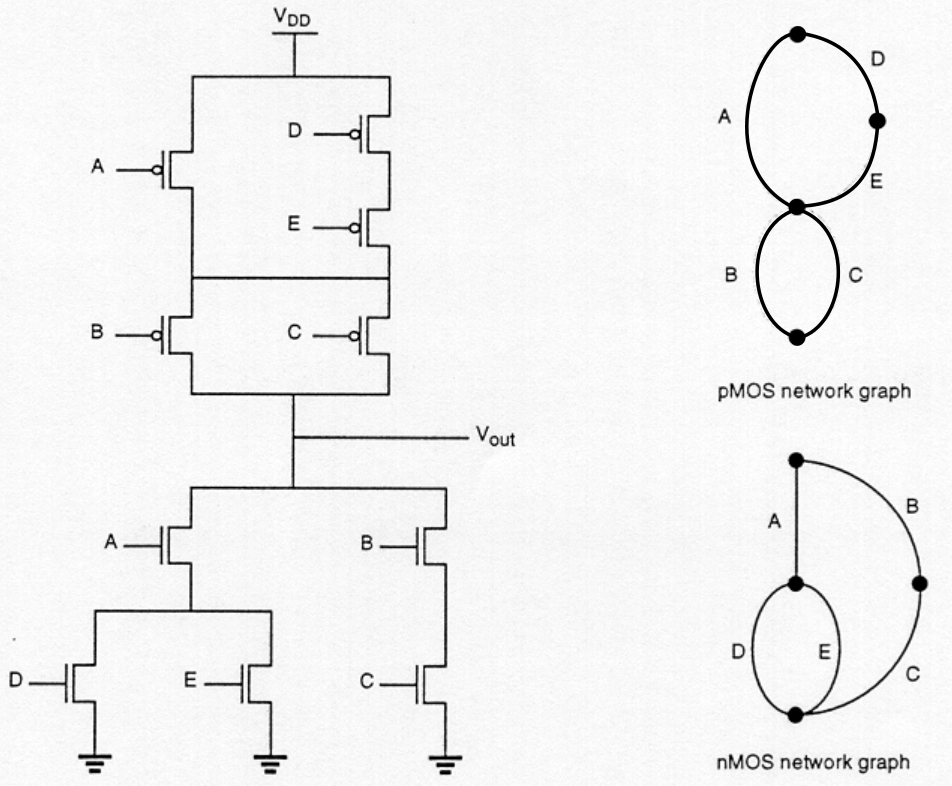
\includegraphics[scale=0.35]{./images/dualite_eulerien.png}
  \end{center}
\end{frame}

% % ------------------------------------------------------------
% \section{Porte NAND}
%
% \begin{frame}{Porte NAND à 2 entrées}
%   \begin{columns}
%     \begin{column}{0.55\textwidth}
%       \begin{circuitikz}[scale=1.0, transform shape]
%         % --- Rail VDD ---
%         \draw (-0.8,5.2) node[above]{$V_{DD}$};
%         \draw (-0.8,5.2) to[short] (1.4,5.2);
%         % --- PMOS A (gauche) et PMOS B (droite), en parallele ---
%         \draw (-0.8,5.2) to[short] (-0.8,4.7);
%         \draw (-0.8,4.7) node[pmos, anchor=S](Pa){};
%         \draw (Pa.G) -- ++(-0.8,0) node[left]{$A$};
%         \draw (1.4,5.2) to[short] (1.4,4.7);
%         \draw (1.4,4.7) node[pmos, anchor=S](Pb){};
%         \draw (Pb.G) -- ++(0.8,0) node[right]{$B$};
%         % --- jonction des deux drains PMOS vers Y ---
%         \draw (Pa.D) to[short] (-0.8,3.8) to[short] (0.3,3.8);
%         \draw (Pb.D) to[short] (1.4,3.8) to[short] (0.3,3.8);
%         \draw (0.3,3.8) to[short] (0.3,3.2);
%         \draw (1.1,3.2) node{$Y$};
%         % --- NMOS A et B en serie ---
%         \draw (0.3,3.2) node[nmos, anchor=D](Na){};
%         \draw (Na.G) -- ++(-0.8,0) node[left]{$A$};
%         \draw (Na.S) to[short] (0.3,1.9);
%         \draw (0.3,1.9) node[nmos, anchor=D](Nb){};
%         \draw (Nb.G) -- ++(-0.8,0) node[left]{$B$};
%         \draw (Nb.S) to[short] (0.3,0.9);
%         \draw (0.3,0.9) node[ground]{};
%       \end{circuitikz}
%     \end{column}
%     \begin{column}{0.45\textwidth}
%       \begin{itemize}
%         \item NMOS $A$ et $B$ en \textbf{série} $\to$ conduit
%           seulement si $A=1$ ET $B=1$
%         \item PMOS $A$ et $B$ en \textbf{parallèle} (dual)
%         \item $Y=0$ uniquement si $A=B=1$
%       \end{itemize}
%       \[ Y = \overline{A \cdot B} \]
%     \end{column}
%   \end{columns}
% \end{frame}


%========================================================================================
\section{Montée en abstraction}
%========================================================================================

\begin{frame}{Conception des Portes logiques : plusieurs niveaux d'abstraction}
  [Guyot TIMA 1995]
  \begin{center}
    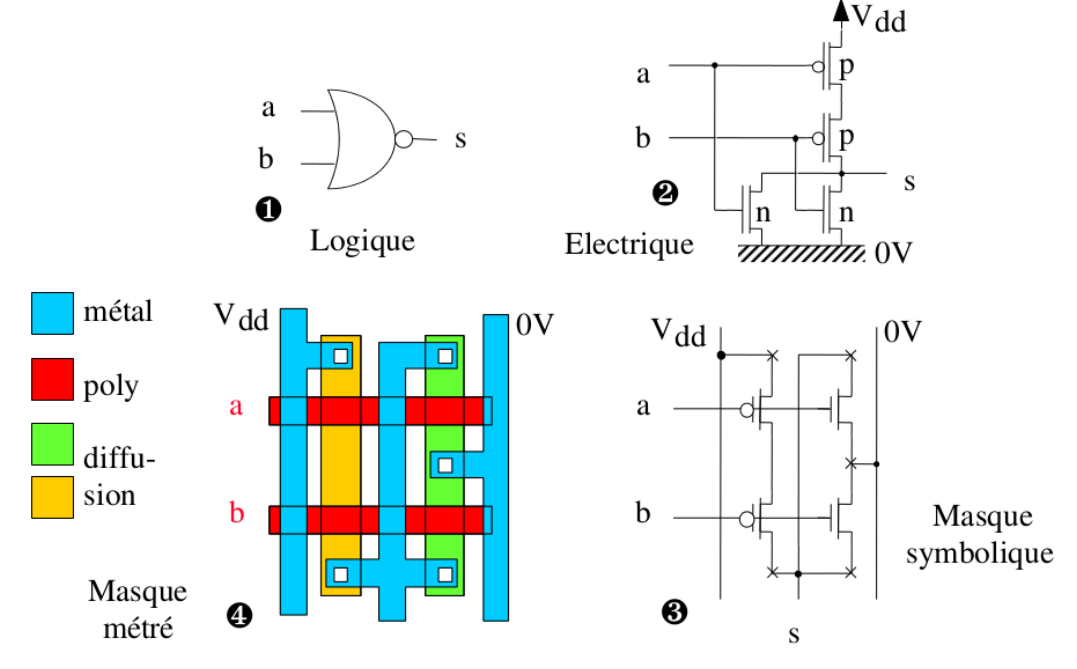
\includegraphics[scale=0.3]{./images/guyot.png}
  \end{center}
\end{frame}


\begin{frame}{Conception des Systèmes numériques : Y de Gajski}

  \begin{columns}[T,onlytextwidth]
    \begin{column}{0.47\textwidth}
      \begin{center}
        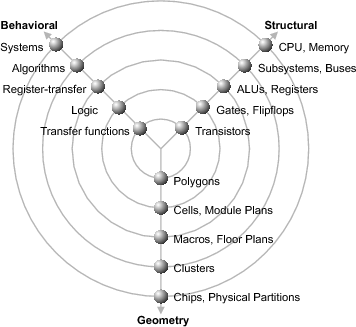
\includegraphics[scale=0.4]{./images/y_gajski.png}
        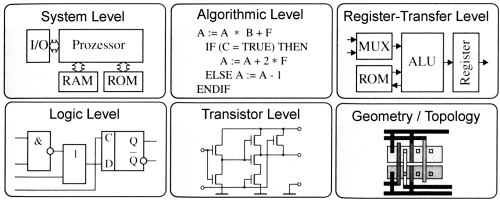
\includegraphics[scale=0.3]{./images/y_gajski_2.png}
      \end{center}
    \end{column}

    \begin{column}{0.51\textwidth}
      \begin{center}
        \includegraphics[scale=0.15]{./images/gajski.jpg}
        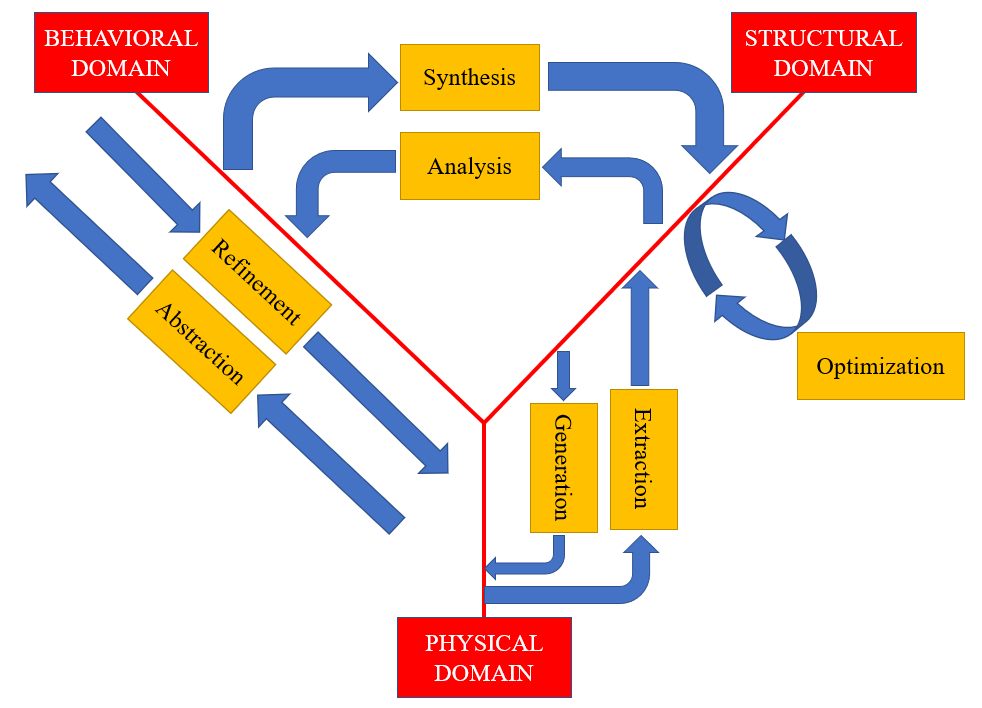
\includegraphics[scale=0.30]{./images/y_gajski_3.png}
      \end{center}
    \end{column}
  \end{columns}

\end{frame}

\begin{frame}{Abstraction et Synthèse automatique}
  \begin{columns}
    \begin{column}{0.50\textwidth}
      \begin{itemize}
        \item Complexité des systèmes
        \item Recours à des langages spécifiques : HDL.
        \begin{itemize}
          \item Description
          \item Simulation (laboratoire virtuel)
          \item Synthèse automatique
        \end{itemize}
        \item ...à différents niveaux d'abstraction.
      \end{itemize}
    \end{column}
    \begin{column}{0.50\textwidth}
      \begin{center}
        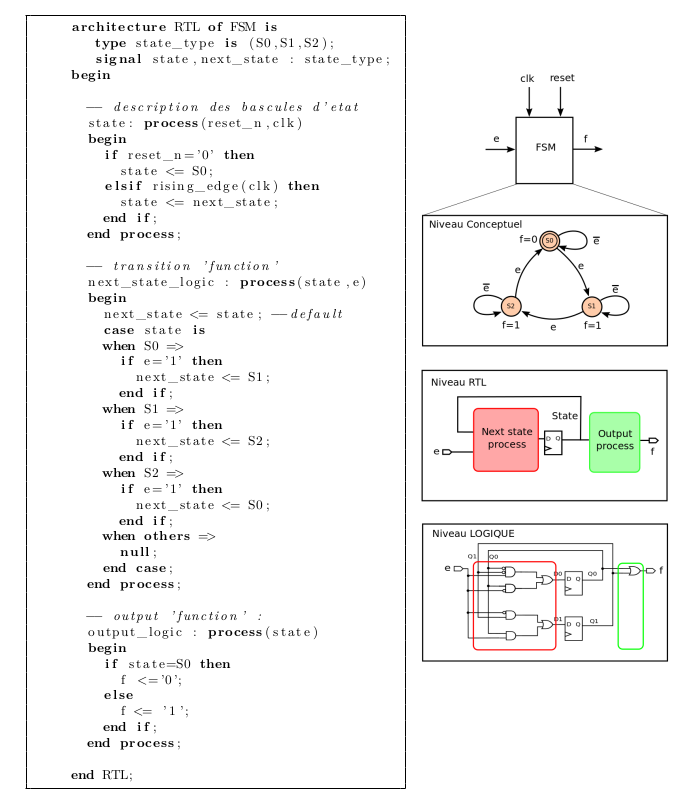
\includegraphics[scale=0.25]{./images/fsm.png}
      \end{center}
    \end{column}
  \end{columns}
\end{frame}

\begin{frame}{Abstractions : système et automates}
  \begin{center}
    \includegraphics[scale=1.0]{./images/gemini_abstraction_soc.jpeg}
  \end{center}
\end{frame}

\begin{frame}{Electronic Design Automation (EDA) : }

  \begin{columns}[T]

    \begin{column}{0.52\textwidth}
      \begin{itemize}
        \setlength{\itemsep}{4pt}
        \item \textbf{Spécification système} : besoins et fonctionnalités
        \item \textbf{Conception architecturale} : partitionnement HW/SW
        \item \textbf{Conception fonctionnelle et RTL} : description HDL (Verilog/VHDL)
        \item \textbf{Synthèse logique} : RTL $\rightarrow$ netlist de portes
        \item \textbf{Conception physique} : placement et routage
        \item \textbf{Vérification physique et signoff} : DRC, LVS, STA
        \item \textbf{Fabrication} : gravure sur wafer (silicium)
        \item \textbf{Packaging et test} : mise en boîtier, tests
        \item \textbf{Puce finale} : circuit intégré prêt à l'emploi
      \end{itemize}
    \end{column}


    \begin{column}{0.44\textwidth}
      \centering
      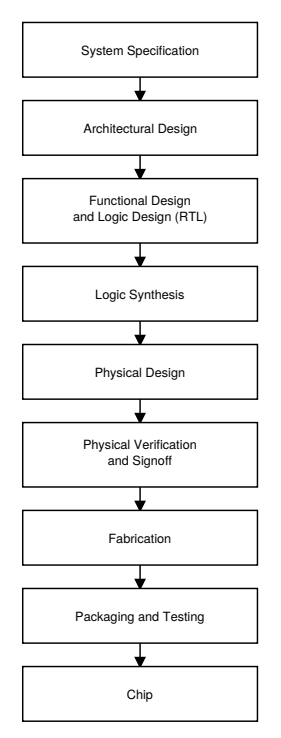
\includegraphics[width=\textwidth,height=0.85\textheight,keepaspectratio]{./images/eda_flow.png}
      %\includesvg[width=\textwidth,height=0.85\textheight,keepaspectratio]{./images/eda_flow.svg}
    \end{column}

  \end{columns}
\end{frame}

\begin{frame}{Du transistor (1947) au \texttt{xeon} d'Intel}
    \begin{center}
        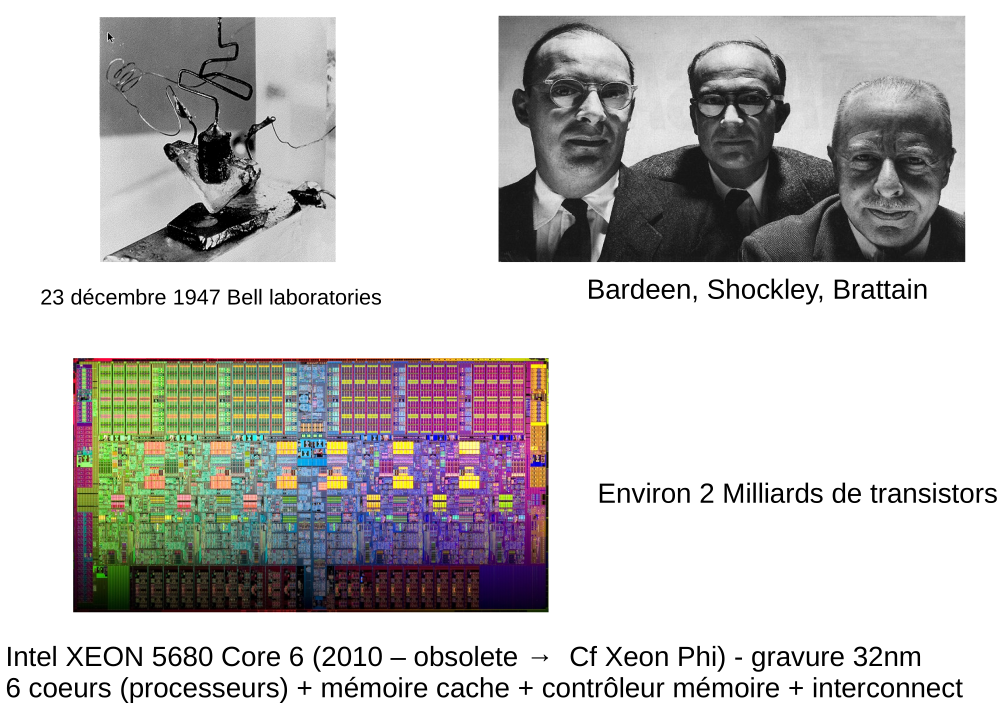
\includegraphics[scale=0.3]{./images/transistor_1947.png}
    \end{center}
\end{frame}

\begin{frame}{Jalons historiques: loi de Moore}
  \begin{columns}[T] % [T] aligne en haut, [c] centré, [b] en bas
    \begin{column}{0.5\textwidth}  % Colonne de gauche (50% de la largeur)
      \begin{itemize}
        \item Doublement du nombre de transistors tous les 18 mois.
      \end{itemize}
      \begin{center}
        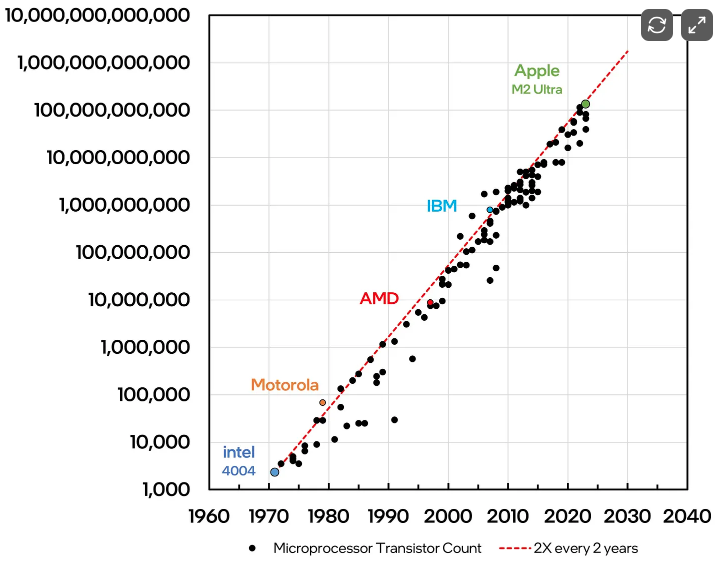
\includegraphics[scale=0.3]{./images/history_moore.png}
      \end{center}
    \end{column}

    \begin{column}{0.5\textwidth}  % Colonne de droite (50% de la largeur)
        \begin{itemize}
        \item Perspective historique plus large.
        \end{itemize}
        \begin{center}
          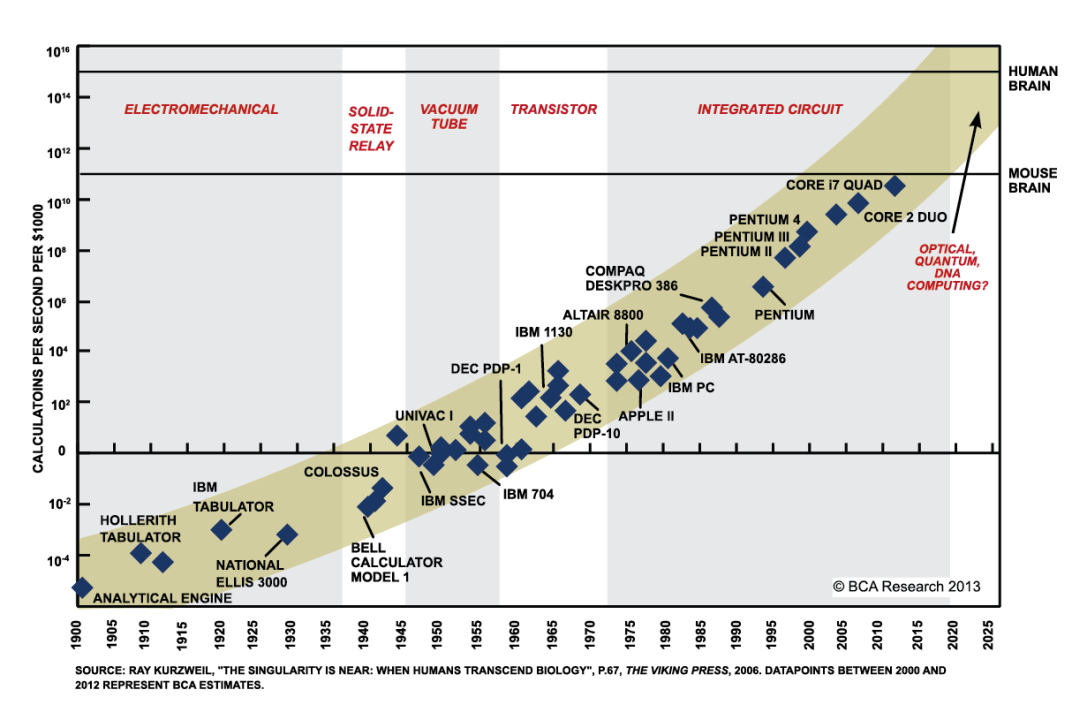
\includegraphics[scale=0.20]{./images/history_1.png}
        \end{center}
        1971 : Intel 4004
    \end{column}
    \end{columns}
\end{frame}

\begin{frame}{Le cas des mémoires :}
    \begin{center}
        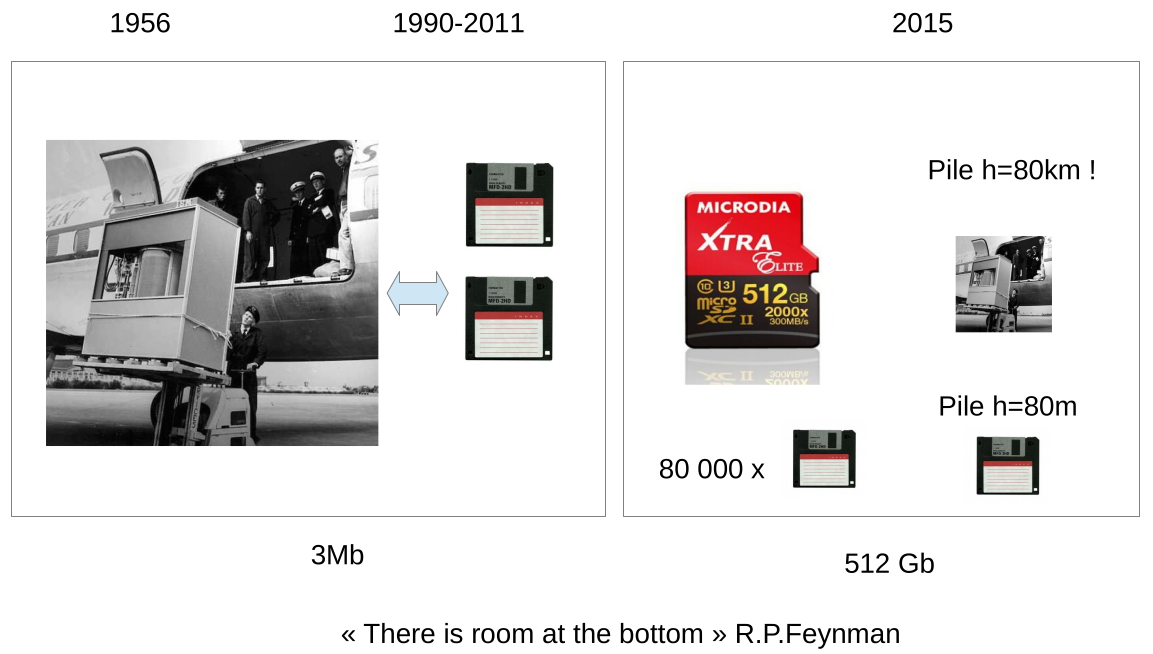
\includegraphics[scale=0.3]{./images/disquette.png}
    \end{center}
\end{frame}


%========================================================================================
\section{Représentations numériques}
%========================================================================================
\begin{frame}{Base de numération}
  \begin{itemize}
    \item On parle de \textit{base} ou \textit{radix} $r$.
    \begin{itemize}
      \item Utilisation des \textit{symboles} de $0$ à $r-1$.
      \item Notation \textit{positionnelle}
      \item Les entiers se décomposent à l'aide des coefficients des puissances de $r$.
    \end{itemize}

    \item Base 10 :
    \begin{itemize}
      \item $142 = 1\times 10^2 + 4 \times 10^1 + 2  \times 10^0$
    \end{itemize}

    \item Base 10, nombres décimaux :
    \begin{itemize}
      \item $142.34 = 1\times 10^2 + 4 \times 10^1 + 2  \times 10^0 + 3 \times 10^{-1} + 4 \times 10^{-2}$
      \item Nombre décimal $\frac{a}{10^n}$ $\rightarrow$ nombre fini de symboles.
      \item Attention : tous les nombres à virgule ne sont pas décimaux !
      \item Attention : lorsqu'on change de base, le nombre de coefficients nécessaires, pour une précision donnée, varie.
      \begin{itemize}
        \item Exemple : $0.2$ ne se représente pas avec un nombre fini de \texttt{bits} dans la base $2$ !
      \end{itemize}

    \end{itemize}
  \end{itemize}
\end{frame}

\begin{frame}{Notations non positionnelles : trois exemples}

\textbf{Chiffres romains} \hfill \textit{(additif, symboles à valeur fixe)}

\smallskip
I = 1, V = 5, X = 10, L = 50, C = 100, D = 500, M = 1000

\smallskip
Exemple : MCMXCIV = 1000 + (1000-100) + (100-10) + (5-1) = \textbf{1994}

\vspace{0.6cm}

\textbf{Système unaire} \hfill \textit{(additif pur, une marque par unité)}

\smallskip
\texttt{|||||} = 5 \qquad \texttt{|||||||} = 7 \quad \textit{(ou groupes de 5)}

\vspace{0.6cm}

\textbf{Hiéroglyphes égyptiens} \hfill \textit{(additif, un symbole par puissance de 10)}

\smallskip
\begin{tabular}{ll}
$\vert$ = 1 & $\cap$ = 10 \\
$\curlywedge$ = 100 & $\odot$ = 1000 \\
\end{tabular}

\smallskip
24 s'écrit : deux « anses » + quatre « traits » --- \textbf{l'ordre n'importe pas}

\vspace{0.4cm}

\centering
\footnotesize\itshape
Dans tous ces systèmes, la position d'un symbole ne modifie jamais sa valeur.

\end{frame}

\begin{frame}{Généralisation}
  La formule générale pour la base 10 est bien entendu :
  $$ x = \sum_{i=-\infty}^{i=+\infty} c_i.10^i, c_i \in \{0,\dots,9 \}$$
  et se généralise :
  $$ \forall r, x = \sum_{i=-\infty}^{i=+\infty} c_{i,r}.r^i, c_{i,r} \in \{0,\dots,(r-1)\}$$
  Lors des changements de base, il faut une notation pour préciser la base de représentation.
  \begin{itemize}
    \item Par exemple : $ 142_{10} = 10001110_{2}$
    \item En logiciel : $ 142_{10} = \text{\texttt{0b10001110}} = \text{\texttt{0x8e}} = \text{\texttt{0o216}}$

    \end{itemize}
\end{frame}

\begin{frame}{Compter en binaire : convertir par table}

  \begin{columns}
    \begin{column}{0.5\textwidth}
      \begin{table}[h]
        \centering
        \resizebox{!}{0.44\textheight}{%
        \begin{tabular}{c|ccccc}
          \toprule
          \multirow{2}{*}{\textbf{Decimal count}} & \multicolumn{5}{c}{\textbf{Binary count}} \\
          \cmidrule(l){2-6} & \textbf{16s} & \textbf{8s} & \textbf{4s} & \textbf{2s} & \textbf{1s} \\
          \midrule
          0  &   &   &   &   & 0 \\
          1  &   &   &   &   & 1 \\
          2  &   &   &   & 1 & 0 \\
          3  &   &   &   & 1 & 1 \\
          4  &   &   & 1 & 0 & 0 \\
          5  &   &   & 1 & 0 & 1 \\
          6  &   &   & 1 & 1 & 0 \\
          7  &   &   & 1 & 1 & 1 \\
          8  &   & 1 & 0 & 0 & 0 \\
          9  &   & 1 & 0 & 0 & 1 \\
          10 &   & 1 & 0 & 1 & 0 \\
          11 &   & 1 & 0 & 1 & 1 \\
          12 &   & 1 & 1 & 0 & 0 \\
          13 &   & 1 & 1 & 0 & 1 \\
          14 &   & 1 & 1 & 1 & 0 \\
          15 &   & 1 & 1 & 1 & 1 \\
          16 & 1 & 0 & 0 & 0 & 0 \\
          17 & 1 & 0 & 0 & 0 & 1 \\
          18 & 1 & 0 & 0 & 1 & 0 \\
          19 & 1 & 0 & 0 & 1 & 1 \\
          \midrule
          & $2^4$ & $2^3$ & $2^2$ & $2^1$ & $2^0$ \\
          \cmidrule(l){2-6}
          & \multicolumn{5}{c}{Powers of 2} \\
          \bottomrule
        \end{tabular}
        % \vspace{1pt}
        % \hspace{2.cm}\textbf{MSB} \hfill \textbf{LSB}\hspace{0.1cm}
        } %resizex
      \end{table}
    \end{column}

    \begin{column}{0.5\textwidth}
      \begin{table}[h]
      \centering
        \resizebox{!}{0.44\textheight}{
        \begin{tabular}{cccc}
        \toprule
        \textbf{Décimal} & \textbf{Binaire} & \textbf{Octal} & \textbf{Hexadécimal} \\
        \midrule
        0  & 0000 & 0  & 0 \\
        1  & 0001 & 1  & 1 \\
        2  & 0010 & 2  & 2 \\
        3  & 0011 & 3  & 3 \\
        4  & 0100 & 4  & 4 \\
        5  & 0101 & 5  & 5 \\
        6  & 0110 & 6  & 6 \\
        7  & 0111 & 7  & 7 \\
        8  & 1000 & 10 & 8 \\
        9  & 1001 & 11 & 9 \\
        10 & 1010 & 12 & A \\
        11 & 1011 & 13 & B \\
        12 & 1100 & 14 & C \\
        13 & 1101 & 15 & D \\
        14 & 1110 & 16 & E \\
        15 & 1111 & 17 & F \\
        \bottomrule
      \end{tabular}
      }
      \end{table}
    \end{column}

  \end{columns}
\end{frame}

\begin{frame}{A quoi ça sert ?}
  \begin{center}
    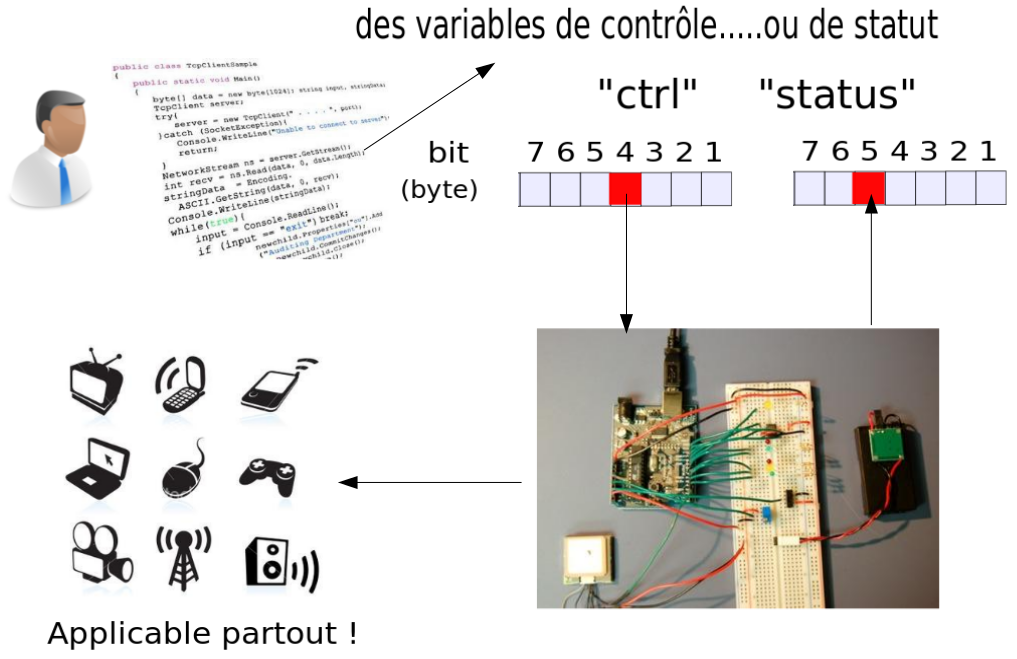
\includegraphics[scale=0.3]{./images/numbers_2.png}
  \end{center}
\end{frame}

\begin{frame}{A quoi ça sert ?}
  \begin{columns}
    \begin{column}{0.5\textwidth}
      \begin{center}
        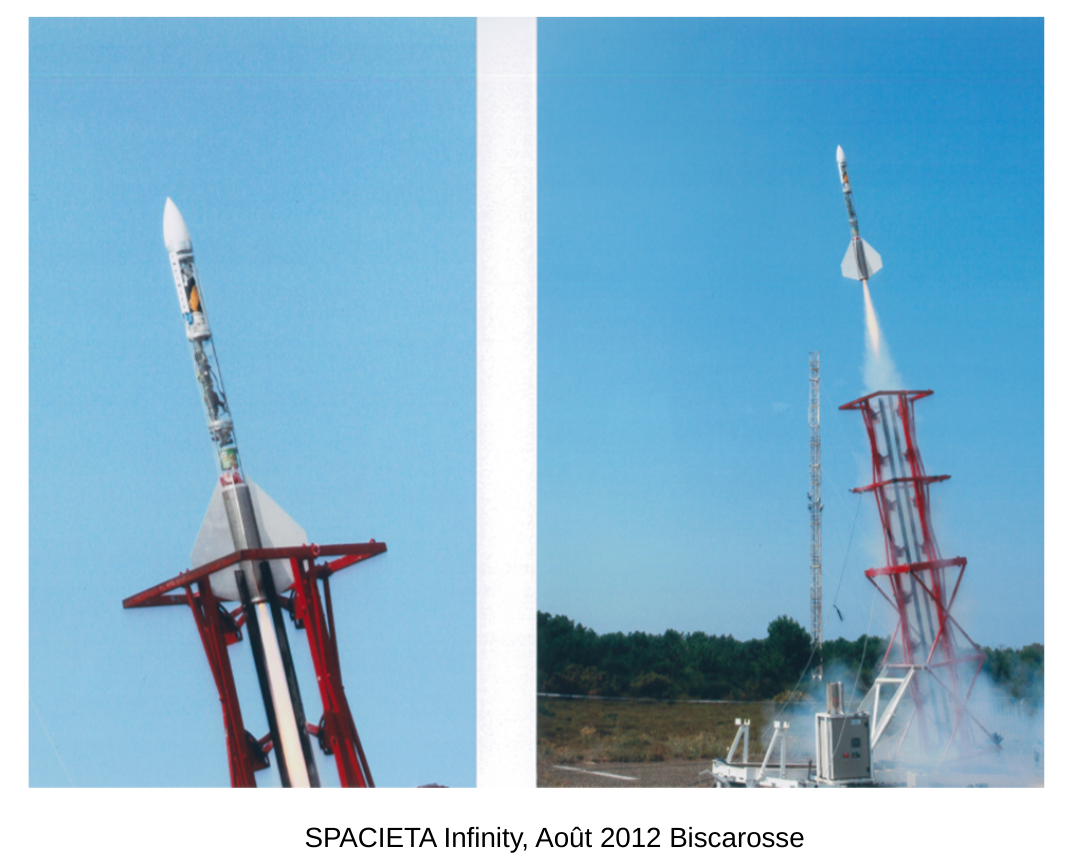
\includegraphics[scale=0.18]{./images/spacieta.png}
      \end{center}
    \end{column}

    \begin{column}{0.5\textwidth}
      \begin{center}
        \includegraphics[scale=0.18]{/home/jcll/Dropbox/IMAGES_TECHNIQUES/JOG.jpg}
      \end{center}
      JOG : conçu  à l'ENSTA Bretagne pour l'enseignement 1A.
    \end{column}
  \end{columns}
\end{frame}

\begin{frame}{Conversions entre bases : par table}
  \begin{center}
    \small $101101_{2} = \text{10\_1101}_{2} = \text{0010\_1101}_{2} = 2D_{16} = \mathbf{0x2D}$
  \end{center}

  \smallskip
  {\small Dans le cas de nombres fractionnaires, on rajoute des 0 à droite de la
  partie fractionnaire. Ainsi~:}

  \begin{center}
    \small le nombre $1011.01_{2} = \text{1011.0100}_{2} = B.4_{16}$
  \end{center}

  \smallskip
  {\small On procède de même pour la traduction octale.}

  \begin{center}
    \small $(10110001101011.1111)_{2} = (\text{101 110 001 101 011}.\text{111 100})_{2} = (36153.74)_{8}$
  \end{center}

  \smallskip
  \begin{center}
    \small
    \begin{tabular}{cccc}
      4 & 7 & . & F \quad E \\[-2pt]
      $\downarrow$ & $\downarrow$ & & $\downarrow$ \qquad $\downarrow$ \\[-2pt]
      0100 & 0111 & . & 1111 \quad 1110
    \end{tabular}

    \smallskip
    \small $47.\text{FE}_{16} \approx 1000111.1111111_{2}$
  \end{center}

\end{frame}

\begin{frame}{Conversions entre bases : par calcul}
  \begin{center}
    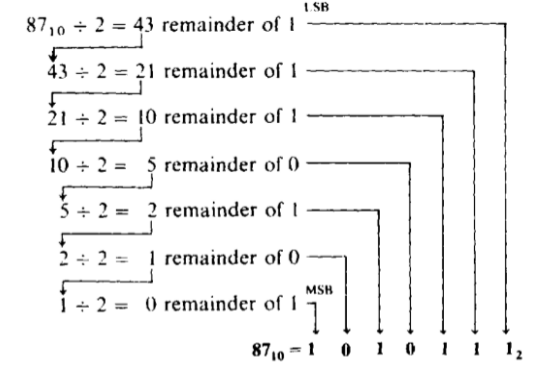
\includegraphics[scale=0.5]{./images/numbers_5.png}
  \end{center}
\end{frame}

\begin{frame}{Conversions entre bases : par calcul}
  \begin{center}
    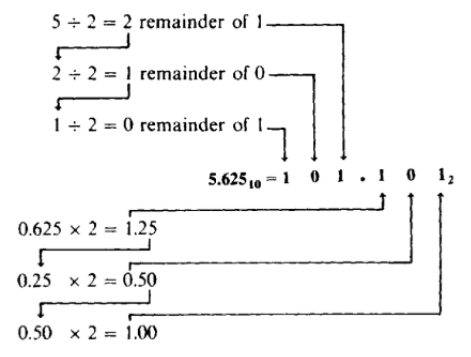
\includegraphics[scale=0.5]{./images/numbers_6.png}
  \end{center}
\end{frame}

\begin{frame}{Conversions entre bases : par calcul}
  \begin{center}
    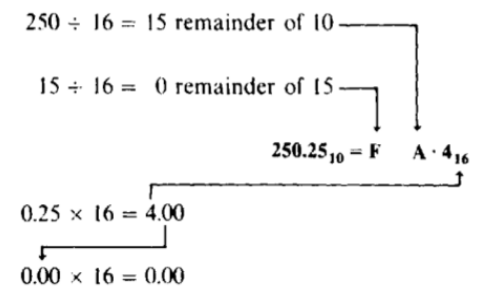
\includegraphics[scale=0.5]{./images/numbers_7.png}
  \end{center}
\end{frame}

\begin{frame}{Autres codes binaires : BCD décimal codé binaire}
  \begin{center}
    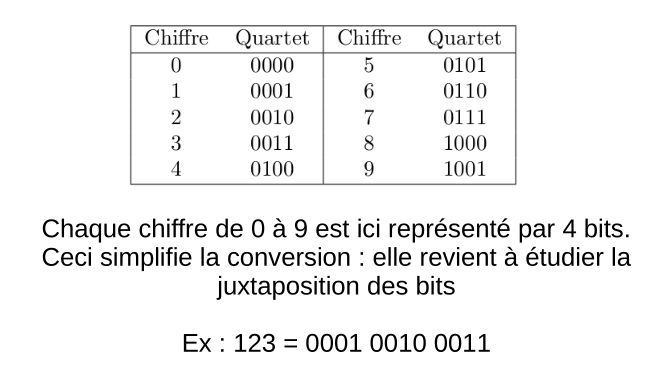
\includegraphics[scale=0.5]{./images/numbers_8.png}
  \end{center}
\end{frame}

\begin{frame}{Autres codes binaires : code de gray ou binaire réfléchi}
  \begin{center}
    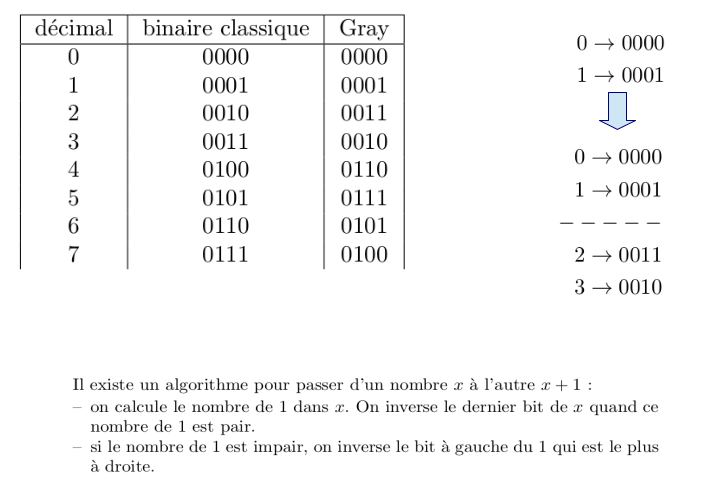
\includegraphics[scale=0.4]{./images/numbers_9.png}
  \end{center}
\end{frame}

\begin{frame}{Entiers positifs ou \texttt{unsigned}}
  \bigskip
  Soit un nombre $W$ de bits et soit $\vec{x} = [x_{w-1},x_{w-2},\ldots,x_0]$ de
  bits. Nous avons vu précédemment (sans la nommer) que la simple fonction~:
  \[
    B2U_w(\vec{x}) \doteq \sum_{i=0}^{w-1} x_i 2^i
  \]
  définit la valeur non-signée ("unsigned") de $\vec{x}$, dans $\mathbb{N}$.
  Les valeurs limites de cette fonction sont~:
  \[
    \begin{cases}
      UMax_w = \sum_{i=0}^{w-1} 2^i = 2^w - 1 \\
      UMmin_w = \sum_{i=0}^{w-1} 0 = 0
    \end{cases}
  \]
  On a donc~:
  \[
    B2U_w : \{0,1\}^w \to \{0,\ldots,2^w-1\}
  \]
\end{frame}

\begin{frame}{Complément à 2 sur w bits}
 \medskip
  \small
  De manière similaire, on définit désormais la fonction qui permet de
  calculer la valeur du vecteur $\vec{x}$ dans le cas d'une valeur signée,
  c'est-à-dire négative ou positive, \textbf{en complément à 2}.
  \[
    B2T_w(\vec{x}) \doteq -x_{w-1}2^{w-1} + \sum_{i=0}^{w-2} x_i 2^i
  \]
  Désormais, le bit de poids fort, le plus à gauche, contribue de manière
  négative à la somme totale. Précisons également que le 'T' vient de
  "two's complement". Calculons les valeurs min et max de cette fonction.
  Pour $\vec{x} = [10\ldots0]$ et $\vec{x} = [01\ldots1]$ respectivement, on
  trouve~:
  \[
    \begin{cases}
      TMin_w = -2^{w-1} \\
      TMax_w = \displaystyle\sum_{i=0}^{w-2} 2^i = 2^{w-1} - 1
    \end{cases}
  \]
  On a donc~:
  \[
    B2U_w : \{0,1\}^w \to \{-2^{w-1},\ldots,2^{w-1}-1\}
  \]
  On pourra également dénoter cette fonction $C_{2,w}(\vec{x})$.
\end{frame}

% ===================================================================
\begin{frame}{Complément à 2 sur w bits}

  \bigskip
  \begin{center}
    \renewcommand{\arraystretch}{1.15}
    \begin{tabular}{|c|c||c|}
      \hline
      \textbf{signé} & \textbf{bit vector} & \textbf{non-signé} \\
      \hline
      $-4$ & 100 & 4 \\ \hline
      $-3$ & 101 & 5 \\ \hline
      $-2$ & 110 & 6 \\ \hline
      $-1$ & 111 & 7 \\ \hline
      $0$  & 000 & 0 \\ \hline
      $1$  & 001 & 1 \\ \hline
      $2$  & 010 & 2 \\ \hline
      $3$  & 011 & 3 \\ \hline
    \end{tabular}
  \end{center}
\end{frame}

% ===================================================================
\begin{frame}{Nombres négatifs}

  \bigskip
  Le complément à 1 d'un nombre binaire consiste à simplement inverser tous
  ses bits.
  \medskip
  Le complément à 2 d'un nombre binaire s'obtient ainsi:
  \begin{itemize}
    \item On parcourt le nombre en partant de la droite (bit de poids faible).
    \item On recopie tel quel tous les bits tant qu'on n'a pas rencontré le premier 1.
    \item On recopie ce premier 1.
    \item On inverse tous les bits suivants (à gauche de ce 1).
  \end{itemize}
  Il existe toutefois une autre méthode, qui se retient plus facilement
  (peut-être). Elle consiste en une formule simple~:

  \bigskip
  \begin{columns}
    \begin{column}{0.35\textwidth}
      \colorbox{blue!20}{\parbox{0.9\textwidth}{\small\textbf{Attention~!!!!}\\
      $-134$ nécessite 9 bits et non 8}}
    \end{column}
    \begin{column}{0.65\textwidth}
      \begin{tikzpicture}
        \node[draw, fill=gray!30, minimum width=3cm, minimum height=1cm, font=\Large] (box) {$-X = \overline{X} + 1$};
        \node[below=0.9cm of box, align=left, xshift=0.3cm] (lab) {\footnotesize Addition classique\\\footnotesize (et non « OU » binaire)};
        \draw[-{Latex[length=3mm]}] (lab.north -| box.south) -- (box.south);
      \end{tikzpicture}
    \end{column}
  \end{columns}
\end{frame}

% ===================================================================
\begin{frame}{Nombres négatifs : représentations obsolètes}
  \bigskip
  \small
  La représentation en magnitude signée est simplement~:
  \[
    B2S_w(\vec{x}) \doteq (-1)^{x_{w-1}} \sum_{i=0}^{w-2} x_i 2^i
  \]
  Il existe également une représentation des nombres en complément à 1,
  très légèrement différente du complément à 2.
  \[
    B2T_w(\vec{x}) \doteq -x_{w-1}(2^{w-1}-1) + \sum_{i=0}^{w-2} x_i 2^i
  \]

  \bigskip
  \begin{center}
    \begin{tikzpicture}
      %\node[arrow, fill=red, minimum height=1cm, arrow head extend=2mm] (arr) {};
      \node[draw, fill=blue!10, align=center] {Ces représentations proposent 2 encodages pour 0~!};
    \end{tikzpicture}
  \end{center}

  \normalsize
  Dans le cas de la magnitude signée~:\\
  $+0 = 0\ldots.0$ et $-0 = 10\ldots0$
\end{frame}

% ===================================================================
\begin{frame}{Nombres négatifs : résumé}
  \begin{columns}[t]
    \begin{column}{0.42\textwidth}
      \tiny
      \renewcommand{\arraystretch}{1.05}
      \begin{tabular}{|c|c|}
        \hline
        \textbf{Signed decimal} & \textbf{8-bit 2's compl.} \\
        \hline
        $+127$ & 0111 1111 \\
        $+126$ & 0111 1110 \\
        $+125$ & 0111 1101 \\
        $\vdots$ & $\vdots$ \\
        $+1$ & 0000 0001 \\
        $+0$ & 0000 0000 \\
        \hline
        $-1$ & 1111 1111 \\
        $-2$ & 1111 1110 \\
        $\vdots$ & $\vdots$ \\
        $-125$ & 1000 0011 \\
        $-126$ & 1000 0010 \\
        $-127$ & 1000 0001 \\
        $-128$ & 1000 0000 \\
        \hline
      \end{tabular}
    \end{column}
    \begin{column}{0.58\textwidth}
      \small
      \begin{center}
        \begin{tikzpicture}
          \node[draw, fill=gray!30, minimum width=2.5cm, minimum height=0.9cm, font=\large] {$-X = \overline{X} + 1$};
        \end{tikzpicture}
      \end{center}

      \bigskip
      \colorbox{orange!40}{
      \begin{minipage}{0.95\textwidth}
        $-125\; ? =$

        \medskip
        $125 \quad = \quad 111\,1101$

        \medskip
        $/125 \quad = \quad \textcolor{red}{1}\,000\,0010$

        \medskip
        $/125+1 = 1\,000\,0011$
      \end{minipage}}
    \end{column}
  \end{columns}

  \bigskip
  \small
  Noter que les nombres en complément à 2 sont négatifs s'ils présentent un
  MSB à 1~!\\
  125 se représente sur 7 bits, mais pas $-125$~: il faut 8 bits
\end{frame}

% ===================================================================
\begin{frame}{\LARGE Exemple~: $-3$ sur 3 bits}


  \begin{columns}[t]
    \begin{column}{0.62\textwidth}
      \begin{itemize}
        \item $3_{10} = 011_2$
        \item $-3_{10} = /3_{10} + 1 = 100_2 + 1 = 101_2 = 5_{10}$~????
        \begin{itemize}
          \item 5 ne peut pas être représenté sur 3 bits, si on y
            représente également les nombres négatifs.
        \end{itemize}
      \end{itemize}

      \bigskip
      \colorbox{blue!30}{\parbox{0.95\textwidth}{\centering
        Pour un nombre donné de bits,\\
        il faut s'entendre sur le fait\\
        que la représentation d'un nombre est signée ou non}}
    \end{column}
    \begin{column}{0.35\textwidth}
      \small
      \begin{tabular}{cc}
        $+3$ & 011 \\
        $+2$ & 010 \\
        $+1$ & 001 \\
        $+0$ & 000 \\
        $-1$ & 111 \\
        $-2$ & 110 \\
        $-3$ & 101 \\
        $-4$ & 100 \\
      \end{tabular}
    \end{column}
  \end{columns}
\end{frame}

% ===================================================================
\begin{frame}{Addition et soustraction}

  \bigskip
  \textbf{Addition}~: classique
  \hfill
  \begin{minipage}{0.55\textwidth}
    \centering
    \renewcommand{\arraystretch}{1.2}
    \begin{tabular}{|l|r|}
      \hline
      & \textbf{Addition} \\
      \hline
      calcul & \begin{tabular}{r}0110\\ $+$0011\end{tabular} \\
      \hline
      retenus & 11 \\
      \hline
      résultat & 1001 \\
      \hline
    \end{tabular}
  \end{minipage}

  \bigskip
  \textbf{Soustraction : x - y}

  \small
  \begin{enumerate}
    \item on additionne $x$ et le complément à 2 de $y$
    \item si le résultat présente une retenue finale, on l'oublie~!
    \item s'il n'y a pas de retenue finale, on prend le complément à 2 du
      résultat et on place un signe "-" devant le nombre.
  \end{enumerate}

  \medskip
  \textbf{exemple}~: $x = 1101100_2$ et $y = 1011011_2$
  \[
    1101100 + 0100101 = 1\,0010001
  \]
  Le résultat est donc $x - y = 0010001_2$

  \hfill\tiny 108-91
\end{frame}

% ===================================================================
\begin{frame}{\LARGE Nombre en virgule fixe : ou \textit{fixed point}}

  \bigskip
  \begin{itemize}
    \item Déjà vu précédemment\ldots
    \item Le calculateur numérique devra connaître la position de la
      virgule, fixée une bonne fois pour toute.
    \item Impact sur les opérations classiques~:
    \begin{itemize}
      \item Le résultat de l'addition hérite de la position de la virgule
        identique à celle dans les opérandes
      \item Cela est changé pour les autres opérations.
    \end{itemize}
  \end{itemize}
\end{frame}

% ===================================================================
\begin{frame}{Nombres en virgule flottante : norme \texttt{ieee754}}

  \begin{center}
    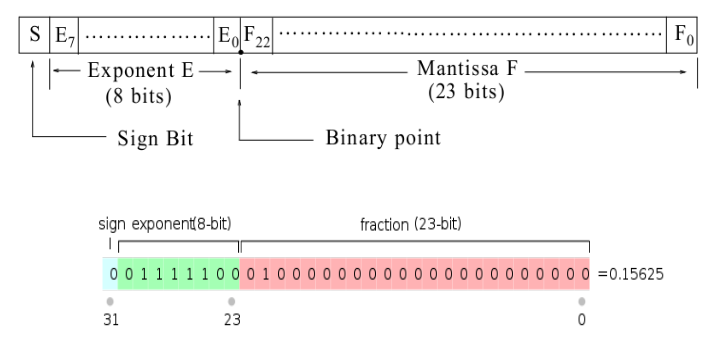
\includegraphics[scale=0.5]{./images/ieee754.png}
  \end{center}

  \bigskip
  \begin{center}
    \begin{tikzpicture}
      \node[single arrow, fill=blue!60, minimum height=1cm, single arrow head extend=2mm] (arr) {};
      \node[draw, fill=blue!10, right=0.2cm of arr] {Exo~: calculer le nombre max et min représentable};
    \end{tikzpicture}
  \end{center}
\end{frame}

% ===================================================================
\begin{frame}{IEEE 754 (SP)}
  \bigskip
  \begin{itemize}
    \item L'exposant est biaisé (en excédent) à 127. C'est-à-dire que pour
      coder un exposant $e$, on code le nombre $e+127$.
    \item Les exposants représentables vont de $-126$ à $127$ (les valeurs
      $00000000$ et $11111111$ sont réservées pour des cas exceptionnels)
    \item Les nombres sont normalisés, c'est-à-dire que la mantisse est
      entre 1 et 2.
  \end{itemize}
\end{frame}

% ===================================================================
\begin{frame}{IEEE 754 : cas exceptionnels}
  \bigskip
  \begin{itemize}
    \item Si $e = 11111111_2$ et $m=0$, le nombre représenté est $+$ ou $-$
      l'infini. Les opérations sur l'infini sont gérées correctement.
    \item Si $e = 11111111_2$ et $m \neq 0$, la représentation est
      considérée comme n'étant pas un nombre (NaN~: Not a Number).
    \item Si $e=0$ et $m=0$ on représente le nombre $+0$ ou $-0$ selon le
      signe.
    \item Si $e=0$ et $m \neq 0$ on dit que le nombre est dénormalisé.
      C'est-à-dire que la mantisse est écrite sans le 1 implicite.
  \end{itemize}
\end{frame}

% ===============================================================
\begin{frame}{Exemple de conversion  vers \texttt{ieee 754}}

  \textbf{Nombre à encoder :} $-12{,}375$

  \vspace{0.3cm}
  \textbf{1. Signe} \; : le nombre est négatif $\Rightarrow s = 1$

  \vspace{0.3cm}
  \textbf{2. Partie entière} \; : $12 = 1100_2$

  \vspace{0.3cm}
  \textbf{3. Partie fractionnaire} \; : $0{,}375$
  \[
    0{,}375 \times 2 = 0{,}75 \rightarrow 0 \qquad
    0{,}75 \times 2 = 1{,}5 \rightarrow 1 \qquad
    0{,}5 \times 2 = 1{,}0 \rightarrow 1
  \]
  \[
    \Rightarrow\; 12{,}375 = 1100{,}011_2
  \]

  \vspace{0.3cm}
  \textbf{4. Normalisation} \; : $\;1100{,}011_2 = 1{,}100011_2 \times 2^{3}$
  \begin{itemize}
    \item Mantisse : $m = 100011$
    \item Exposant réel : $e = 3$
    \item Exposant biaisé : $E = 3 + 127 = 130 = 10000010_2$
  \end{itemize}
\end{frame}

% ===============================================================
\begin{frame}{Étape 3 : assemblage des 32 bits}

  \begin{center}
  \begin{tikzpicture}[scale=0.85]
    \draw[fill=blue!20] (0,0) rectangle (1,0.8);
    \node at (0.5,0.4) {1};

    \draw[fill=green!20] (1,0) rectangle (5,0.8);
    \node at (3,0.4) {1000\,0010};

    \draw[fill=orange!20] (5,0) rectangle (11,0.8);
    \node at (8,0.4) {1000\,1100\,0000\,0000\,0000\,000};

    \node at (0.5,-0.35) {\small $s$};
    \node at (3,-0.35)   {\small exposant};
    \node at (8,-0.35)   {\small mantisse};
  \end{tikzpicture}
  \end{center}

  \vspace{0.4cm}
  \begin{block}{Résultat final}
    \[
      -12{,}375 \;\longrightarrow\;
      \underbrace{1}_{\text{signe}}\;
      \underbrace{10000010}_{\text{exposant}}\;
      \underbrace{10001100000000000000000}_{\text{mantisse}}
    \]
    \[
      \boxed{\texttt{0xC1460000}} \quad \text{(hexadécimal)}
    \]
  \end{block}

  \vspace{0.3cm}
  \textbf{Vérification :} $(-1)^1 \times 1{,}100011_2 \times 2^{130-127} = -12{,}375$ \checkmark
\end{frame}

\begin{frame}{\texttt{IEEE 754} : l'addition n'est pas commutative !}
  \begin{alertblock}{Avertissement}
    En arithmétique flottante IEEE 754, à cause des \textbf{arrondis},
    l'addition \textbf{n'est pas associative}, et dans certains cas elle
    peut même sembler \textbf{non commutative} lorsqu'on enchaîne
    plusieurs opérations ou qu'on change l'ordre des termes.
  \end{alertblock}

  \vspace{0.4cm}
  \textbf{Cause principale :} quand on additionne deux nombres d'ordres
  de grandeur très différents, le plus petit peut être \emph{entièrement
  absorbé} par l'arrondi du plus grand (\emph{absorption} / \emph{swamping}).

  \vspace{0.4cm}
  \begin{block}{Exemple classique en double précision}
    \[
      a = 1{,}0 \qquad b = 2^{-53} \qquad c = 2^{-53}
    \]
    \[
      (a + b) + c \;\neq\; a + (b + c)
    \]
  \end{block}

  \vspace{0.3cm}
  \centering
  \textit{L'ordre des opérations change le résultat !}
\end{frame}
\begin{frame}{Comment s'additionne-t-on deux flottants ?}
  \textbf{Algorithme matériel} (simplifié) pour $x + y$ :

  \vspace{0.4cm}
  \begin{enumerate}
    \item \textbf{Aligner les exposants} : on réécrit le plus petit
      exposant pour qu'il coïncide avec le plus grand. Les bits de sa
      mantisse sont \textbf{décalés vers la droite} — et les bits qui
      « sortent » sont \textbf{perdus}.
    \item \textbf{Additionner les mantisses} (avec le bit implicite).
    \item \textbf{Renormaliser} le résultat si nécessaire.
    \item \textbf{Arrondir} au format (au pair, par défaut).
  \end{enumerate}

  \vspace{0.4cm}
  \begin{block}{Le point critique}
    C'est à l'étape \textbf{1} que se joue tout le drame :
    si les exposants diffèrent de plus de $p$ bits (où $p$ est la
    précision), le plus petit nombre est \textbf{totalement
    sacrifié} au profit du plus grand.
  \end{block}

  % \vspace{0.2cm}
  % \centering
  % \begin{tikzpicture}[scale=0.9, every node/.style={font=\small}]
  %   \node[draw, rounded corners, fill=blue!10, inner sep=6pt] (x)
  %     {$x = 1{,}000\ldots0 \times 2^{0}$};
  %   \node[draw, rounded corners, fill=orange!10, inner sep=6pt,
  %         right=2cm of x] (y)
  %     {$y = 1{,}000\ldots0 \times 2^{-53}$};
  %   \draw[->, thick] (y.south) to[bend right=25]
  %     node[below, font=\scriptsize]{décalage de 53 bits vers la droite}
  %     (x.south);
  % \end{tikzpicture}
\end{frame}

% ===============================================================
\begin{frame}{\texttt{IEEE 754} : Illustration numérique}

  \textbf{Hypothèses :} double précision, $\varepsilon_{\text{mach}} = 2^{-52}$.
  Le plus petit incrément représentable autour de $1{,}0$ est
  $\text{ulp}(1) = 2^{-52}$.

  \vspace{0.4cm}
  \begin{columns}[T]
    \begin{column}{0.48\textwidth}
      \begin{block}{Calcul de $(a+b)+c$}
        \[
          a + b = 1{,}0 + 2^{-53}
        \]
        Or $2^{-53} = \tfrac{1}{2}\,\text{ulp}(1)$, donc l'arrondi
        (au pair) donne :
        \[
          a + b = 1{,}0
        \]
        Puis :
        \[
          (a+b) + c = 1{,}0
        \]
      \end{block}
    \end{column}

    \begin{column}{0.48\textwidth}
      \begin{block}{Calcul de $a+(b+c)$}
        \[
          b + c = 2^{-53} + 2^{-53} = 2^{-52}
        \]
        Cet incrément vaut exactement $\text{ulp}(1)$, donc il est
        représentable :
        \[
          a + (b+c) = 1{,}0 + 2^{-52}
        \]
      \end{block}
    \end{column}
  \end{columns}

  \vspace{0.2cm}
  \begin{center}
    \begin{tikzpicture}
      \node[draw, rounded corners, fill=red!15, inner sep=8pt] {
        $(a+b)+c = 1{,}0 \qquad \neq \qquad a+(b+c) = 1{,}0 + 2^{-52}$
      };
    \end{tikzpicture}
  \end{center}

  \vspace{0.3cm}
  \begin{alertblock}{À retenir}
    Ne jamais tester l'égalité de deux calculs flottants pour une prise de décision.
  \end{alertblock}
\end{frame}


\begin{frame}{Douglas Hofstadter et les « faux » nombres réels}

  \begin{columns}[c]
    \begin{column}{0.28\textwidth}
      \centering
      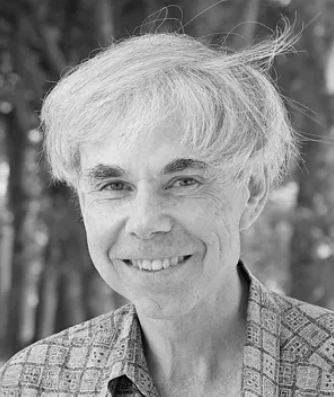
\includegraphics[scale=0.3]{./images/hofstadter.png}

      \vspace{0.2cm}
      {\scriptsize
        Douglas Hofstadter (1945--)\\
        \textit{Gödel, Escher, Bach}\\
        Prix Pulitzer 1980
      }
    \end{column}

    \begin{column}{0.70\textwidth}
      \begin{block}{}
        \itshape
        « En informatique, il n'y a pas de nombres réels. Il n'y a que
        des nombres flottants, et ils sont à peu près aussi réels que
        les personnages de dessins animés. »
      \end{block}

      \vspace{0.3cm}
      \small
      IEEE 754 ne code qu'un \textbf{ensemble fini} de valeurs, et
      chaque opération introduit un \textbf{arrondi}. Pourtant, cette
      arithmétique approximative pilote avions, réacteurs et ponts :
      la fiabilité vient des \textbf{algorithmes}, pas des nombres.
    \end{column}
  \end{columns}
\end{frame}

%============================================================================
\begin{frame}{Représentation des données symboliques}
  Certaines données ne sont pas numériques
  \begin{itemize}
    \item Enumérations, collections : couleurs,alphabets,...
    \item Ou compositions de données numériques
  \end{itemize}
Un encodage de ces données est nécessaire.
  \begin{center}
    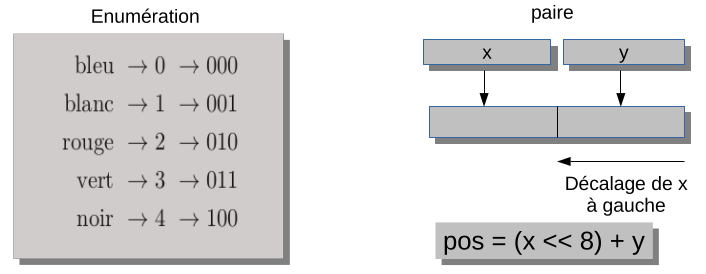
\includegraphics[scale=0.5]{./images/symb_0.png}
  \end{center}
\end{frame}

\begin{frame}{Représentation des données : codes \texttt{ASCII}}
  \begin{center}
    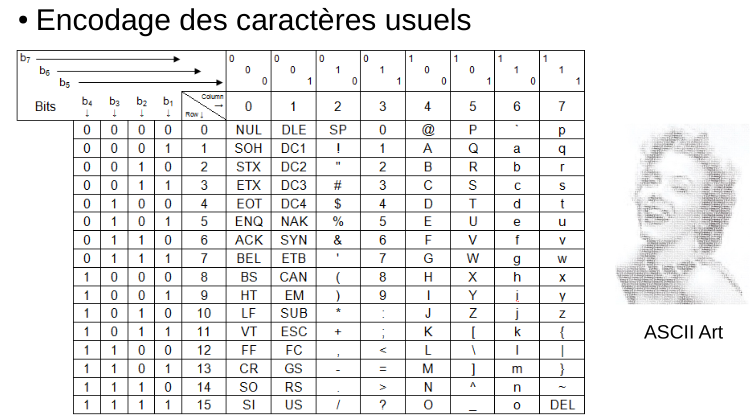
\includegraphics[scale=0.5]{./images/symb_1.png}
  \end{center}
\end{frame}

\begin{frame}{Représentation des données : codes \texttt{UTF8}}
  \begin{center}
    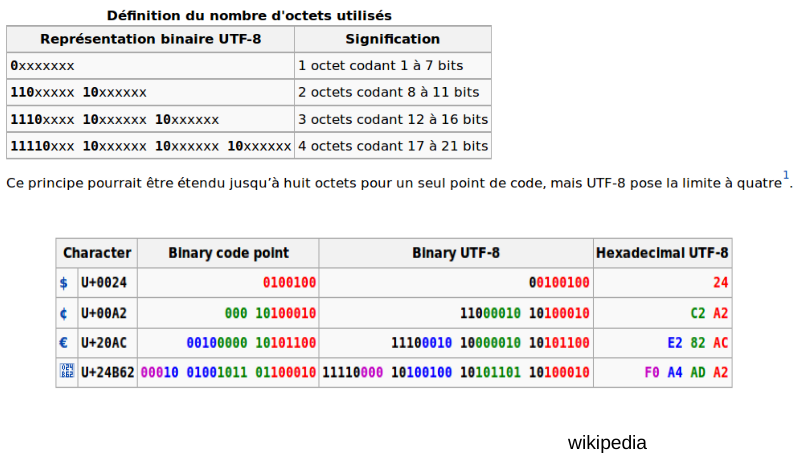
\includegraphics[scale=0.5]{./images/symb_2.png}
  \end{center}
\end{frame}

\begin{frame}{Manipulations binaires \textit{bitwise} : exemple}
  \begin{center}
    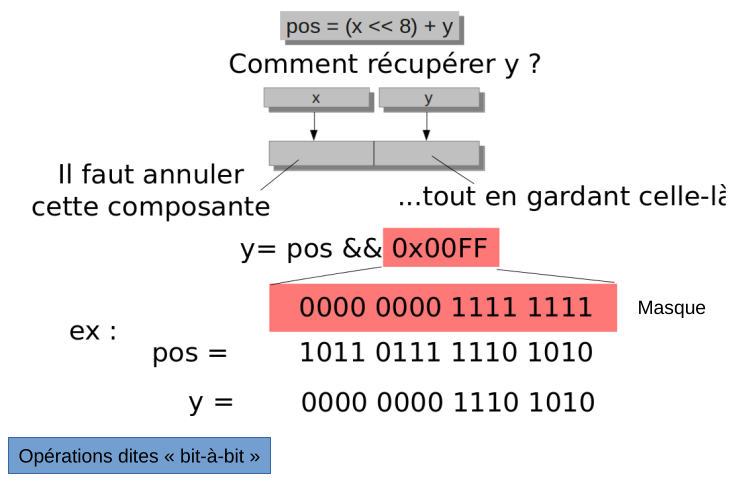
\includegraphics[scale=0.5]{./images/symb_4.png}
  \end{center}
\end{frame}

\begin{frame}{Manipulations binaires \textit{bitwise} traditionnelles}
  \begin{center}
    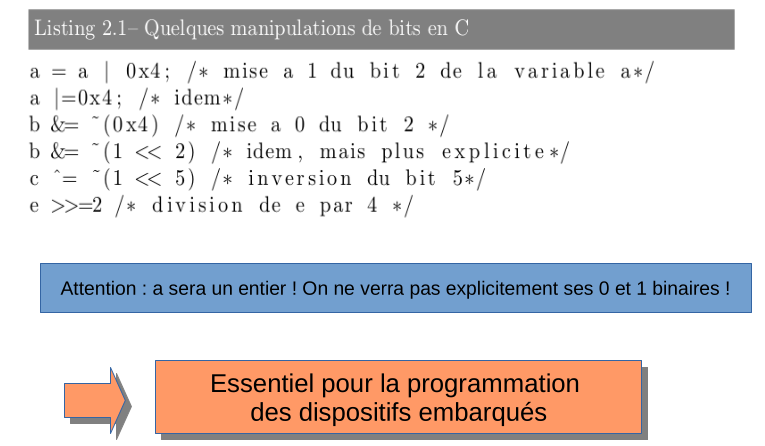
\includegraphics[scale=0.4]{./images/symb_6.png}
  \end{center}
\end{frame}

\begin{frame}{Codes détecteurs d'erreurs}
  \begin{center}
    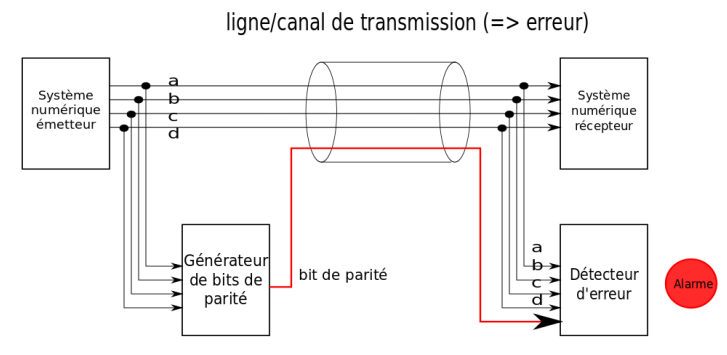
\includegraphics[scale=0.5]{./images/symb_7.png}
  \end{center}
\end{frame}

\begin{frame}{Codes détecteurs d'erreurs}
  \begin{center}
    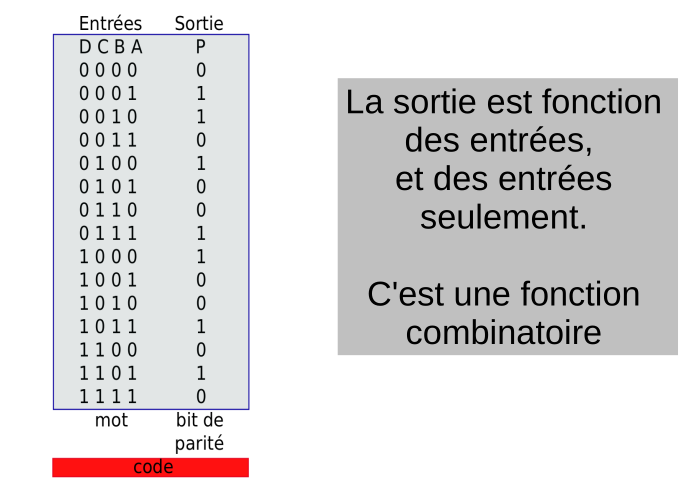
\includegraphics[scale=0.4]{./images/symb_8.png}
  \end{center}
\end{frame}

\begin{frame}{Claude Berrou et les turbocodes : correcteurs d'erreurs}

  \begin{columns}[c]
    \begin{column}{0.68\textwidth}
      \begin{block}{Une révolution née à Brest }
        \itshape
        En 1993, Claude Berrou et Alain Glavieux (ENST/IMT Atlantique) bouleversent la théorie
        de l'information en s'approchant de la \textbf{limite de Shannon},
        que les experts jugeaient inatteignable depuis 1948.
      \end{block}

      \vspace{0.3cm}
      \small
      Les \textbf{turbocodes} reposent sur un principe itératif :
      deux décodeurs élémentaires s'échangent des « croyances »
      jusqu'à converger vers le message original.

      \vspace{0.3cm}
      \textbf{Aujourd'hui :} 3G/4G, WiMAX, sondes spatiales
      (Mars Reconnaissance Orbiter, Messenger), plus de
      \textbf{4 milliards} de turbodécodeurs en circulation.
    \end{column}

    \begin{column}{0.28\textwidth}
      \centering
      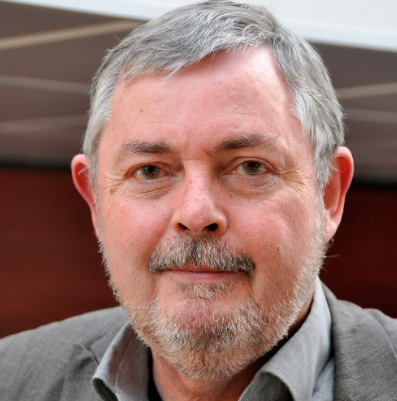
\includegraphics[scale=0.25]{./images/berrou.png}
      \vspace{0.2cm}
      {\scriptsize
        Claude Berrou (1951--)\\
        Télécom Bretagne\\
        Prix Marconi 2005\\
        Médaille Hamming 2003
      }
    \end{column}
  \end{columns}

\end{frame}


%========================================================================================
%\section{Logique Booléenne et Combinatoire}
%========================================================================================
%

% =========================================================
\section{Algèbre de Boole}
% =========================================================

% --- Espace de Boole et variables ---
\begin{frame}{Espace de Boole et Variables Booléennes}

    \begin{block}{L'Espace de Boole \(\mathbb{B}\)}
        L'algèbre booléenne \footnote{L’algèbre de Boole est une algèbre au sens de structure algébrique, mais pas au sens d’algèbre sur un corps $\mathbb{K}$.} opère sur un ensemble à deux éléments :
        \[
            \mathbb{B} = \{0, 1\}
        \]
        où \(0\) représente \textbf{Faux} et \(1\) représente \textbf{Vrai}.
    \end{block}

    \vspace{0.4cm}

    \begin{columns}[T]
        \begin{column}{0.48\textwidth}
            \textbf{Variable booléenne simple}
            \begin{itemize}
                \item Une variable \(x\) qui ne peut prendre que deux valeurs.
                \item \(x \in \{0, 1\}\)
                \item Exemple : \textit{Un interrupteur est ouvert (0) ou fermé (1).}
            \end{itemize}
        \end{column}
        \begin{column}{0.48\textwidth}
            \textbf{Variable booléenne générale (vecteur)}
            \begin{itemize}
                \item Un vecteur de \(n\) bits : \(X = (x_{n-1}, \dots, x_0)\)
                \item \(X \in \mathbb{B}^n\)
                \item Exemple : \textit{Un octet (8 bits) représentant un état.}
            \end{itemize}
        \end{column}
    \end{columns}

\end{frame}

% --- Fonction booléenne ---
\begin{frame}{Fonction Booléenne}

    \begin{block}{Définition}
        Une \textbf{fonction booléenne} à \(n\) variables est une application :
        \[
            f : \mathbb{B}^n \to \mathbb{B}
        \]
        Elle associe à chaque combinaison d'entrées une unique sortie binaire.
    \end{block}

    \vspace{0.4cm}

    \begin{columns}[T]
        \begin{column}{0.55\textwidth}
            \textbf{Représentation}
            \begin{itemize}
                \item \textbf{Table de vérité} : énumère les \(2^n\) cas possibles.
                \item \textbf{Expression algébrique} : combinaison de \(+, \cdot, \bar{\phantom{x}}\).
            \end{itemize}

            \vspace{0.3cm}
            \textit{Exemple :} \(f(x,y) = x \cdot \bar{y} + \bar{x} \cdot y\) (XOR)
        \end{column}
        \begin{column}{0.4\textwidth}
            \centering
            \begin{tabular}{|c|c|c|}
                \hline
                \(x\) & \(y\) & \(f(x,y)\) \\
                \hline
                0 & 0 & 0 \\
                0 & 1 & 1 \\
                1 & 0 & 1 \\
                1 & 1 & 0 \\
                \hline
            \end{tabular}
        \end{column}
    \end{columns}

\end{frame}

% =========================================================
\section{Opérations}
% =========================================================

% --- Opérations fondamentales ---
\begin{frame}{Opérations Fondamentales}

    On utilise usuellement les symboles \(+\) pour le \textbf{OU} et \(\cdot\) (ou \(*\)) pour le \textbf{ET}.

    \vspace{0.3cm}

    \begin{columns}[T]
        \begin{column}{0.3\textwidth}
            \centering
            \textbf{Négation (NON)}\\
            \(\bar{x}\) ou \(\neg x\)
            \vspace{0.2cm}

            \begin{tabular}{|c|c|}
                \hline
                \(x\) & \(\bar{x}\) \\
                \hline
                0 & 1 \\
                1 & 0 \\
                \hline
            \end{tabular}
        \end{column}

        \begin{column}{0.35\textwidth}
            \centering
            \textbf{Conjonction (ET)}\\
            \(x \cdot y\) ou \(x * y\)
            \vspace{0.2cm}

            \begin{tabular}{|c|c|c|}
                \hline
                \(x\) & \(y\) & \(x \cdot y\) \\
                \hline
                0 & 0 & 0 \\
                0 & 1 & 0 \\
                1 & 0 & 0 \\
                1 & 1 & 1 \\
                \hline
            \end{tabular}
        \end{column}

        \begin{column}{0.35\textwidth}
            \centering
            \textbf{Disjonction (OU)}\\
            \(x + y\)
            \vspace{0.2cm}

            \begin{tabular}{|c|c|c|}
                \hline
                \(x\) & \(y\) & \(x + y\) \\
                \hline
                0 & 0 & 0 \\
                0 & 1 & 1 \\
                1 & 0 & 1 \\
                1 & 1 & 1 \\
                \hline
            \end{tabular}
        \end{column}
    \end{columns}

\end{frame}

% --- Opérateurs dérivés (aperçu) ---
\begin{frame}{Opérateurs Dérivés}

    Au-delà des trois opérations de base (\(+, \cdot, \bar{\phantom{x}}\)), on définit des \textbf{opérateurs dérivés} très utilisés en logique et en électronique.

    \vspace{0.4cm}

    \centering
    \begin{tabular}{|c|c|c|}
        \hline
        \textbf{Nom} & \textbf{Symbole} & \textbf{Expression en base} \\
        \hline
        OU exclusif (XOR) & \(x \oplus y\) & \(x \cdot \bar{y} + \bar{x} \cdot y\) \\
        NAND & \(x \uparrow y\) & \(\overline{x \cdot y}\) \\
        NOR & \(x \downarrow y\) & \(\overline{x + y}\) \\
        Équivalence (XNOR) & \(x \Leftrightarrow y\) & \(x \cdot y + \bar{x} \cdot \bar{y}\) \\
        Implication & \(x \Rightarrow y\) & \(\bar{x} + y\) \\
        \hline
    \end{tabular}

    \vspace{0.5cm}

    \begin{block}{Idée clé}
        Tous ces opérateurs se ramènent aux trois opérations fondamentales.
    \end{block}

\end{frame}

% --- XOR ---
\begin{frame}{Le OU Exclusif (\(x \oplus y\))}

    \begin{block}{Définition}
        « \(x\) ou \(y\), mais pas les deux » — noté \(x \oplus y\).
        \[
            x \oplus y \;=\; x \cdot \bar{y} + \bar{x} \cdot y
        \]
    \end{block}

    \vspace{0.4cm}

    \begin{columns}[T]
        \begin{column}{0.42\textwidth}
            \centering
            \begin{tabular}{|c|c|c|}
                \hline
                \(x\) & \(y\) & \(x \oplus y\) \\
                \hline
                0 & 0 & 0 \\
                0 & 1 & 1 \\
                1 & 0 & 1 \\
                1 & 1 & 0 \\
                \hline
            \end{tabular}
        \end{column}
        \begin{column}{0.55\textwidth}
            \textbf{Propriétés utiles :}
            \begin{itemize}
                \item \(x \oplus x = 0\)
                \item \(x \oplus \bar{x} = 1\)
                \item \(x \oplus 0 = x\)
                \item \(x \oplus 1 = \bar{x}\)
                \item \textbf{Associatif et commutatif}
            \end{itemize}

            \vspace{0.2cm}
            \textit{Application : addition binaire, détection de parité.}
        \end{column}
    \end{columns}

\end{frame}

% --- NAND et NOR ---
\begin{frame}{NAND et NOR : les Portes Universelles}

    \begin{columns}[T]
        \begin{column}{0.48\textwidth}
            \begin{block}{NAND (\(x \uparrow y\))}
                \[
                    x \uparrow y = \overline{x \cdot y}
                \]
                \centering
                \begin{tabular}{|c|c|c|}
                    \hline
                    \(x\) & \(y\) & \(x \uparrow y\) \\
                    \hline
                    0 & 0 & 1 \\
                    0 & 1 & 1 \\
                    1 & 0 & 1 \\
                    1 & 1 & 0 \\
                    \hline
                \end{tabular}
            \end{block}
        \end{column}

        \begin{column}{0.48\textwidth}
            \begin{block}{NOR (\(x \downarrow y\))}
                \[
                    x \downarrow y = \overline{x + y}
                \]
                \centering
                \begin{tabular}{|c|c|c|}
                    \hline
                    \(x\) & \(y\) & \(x \downarrow y\) \\
                    \hline
                    0 & 0 & 1 \\
                    0 & 1 & 0 \\
                    1 & 0 & 0 \\
                    1 & 1 & 0 \\
                    \hline
                \end{tabular}
            \end{block}
        \end{column}
    \end{columns}

    \vspace{0.4cm}

    \begin{alertblock}{Universalité}
        Toute fonction booléenne peut être réalisée en n'utilisant \textbf{que des NAND} ou \textbf{que des NOR}.
    \end{alertblock}

\end{frame}
% --- Équivalence ---
\begin{frame}{L'Équivalence (\(x \Leftrightarrow y\))}

    \begin{block}{Définition}
        « \(x\) si et seulement si \(y\) » — notée \(x \Leftrightarrow y\), également écrite \(x \leftrightarrow y\) ou XNOR.
        \[
            x \Leftrightarrow y \;=\; x \cdot y + \bar{x} \cdot \bar{y}
        \]
    \end{block}

    \vspace{0.4cm}

    \begin{columns}[T]
        \begin{column}{0.42\textwidth}
            \centering
            \begin{tabular}{|c|c|c|}
                \hline
                \(x\) & \(y\) & \(x \Leftrightarrow y\) \\
                \hline
                0 & 0 & 1 \\
                0 & 1 & 0 \\
                1 & 0 & 0 \\
                1 & 1 & 1 \\
                \hline
            \end{tabular}
        \end{column}
        \begin{column}{0.55\textwidth}
            \textbf{Points à retenir :}
            \begin{itemize}
                \item Vraie quand \(x\) et \(y\) sont \textbf{identiques}.
                \item C'est la \textbf{négation du XOR}.
                \item \(x \Leftrightarrow y = \overline{x \oplus y}\)
            \end{itemize}

            \vspace{0.3cm}
            \textit{Lien avec l'implication :}
            \[
                (x \Rightarrow y) \cdot (y \Rightarrow x) = x \Leftrightarrow y
            \]
        \end{column}
    \end{columns}

\end{frame}

% --- Implication : définition ---
\begin{frame}{L'Implication (\(x \Rightarrow y\)) : Définition}

    \begin{block}{Définition}
        « Si \(x\) alors \(y\) » — notée \(x \Rightarrow y\) ou \(x \to y\).
        \[
            x \Rightarrow y \;=\; \bar{x} + y
        \]
    \end{block}

    \vspace{0.4cm}

    \begin{columns}[T]
        \begin{column}{0.42\textwidth}
            \centering
            \begin{tabular}{|c|c|c|}
                \hline
                \(x\) & \(y\) & \(x \Rightarrow y\) \\
                \hline
                0 & 0 & 1 \\
                0 & 1 & 1 \\
                1 & 0 & \textbf{0} \\
                1 & 1 & 1 \\
                \hline
            \end{tabular}
        \end{column}
        \begin{column}{0.55\textwidth}
            \textbf{Un seul cas rend l'implication fausse :}
            \[
                x = 1 \quad \text{et} \quad y = 0
            \]

            \vspace{0.3cm}
            C'est le seul \textbf{contre-exemple} possible : l'antécédent est vrai mais la conclusion ne l'est pas.
        \end{column}
    \end{columns}

    \vspace{0.3cm}
    \centering
    \textit{Reformulation : \(x \Rightarrow y = \overline{x \cdot \bar{y}}\)\quad (négation d'un contre-exemple).}

\end{frame}

% --- Implication : paradoxe de l'antécédent faux ---
\begin{frame}{Implication : pourquoi est-elle vraie quand \(x = 0\) ?}

    \begin{alertblock}{La difficulté}
        Intuitivement, on se demande pourquoi \(0 \Rightarrow 0\) et \(0 \Rightarrow 1\) valent \(1\).
    \end{alertblock}

    \vspace{0.3cm}

    \textbf{Clé :} l'implication est une \textbf{contrainte conditionnelle}.

    \vspace{0.2cm}

    \[
        x \Rightarrow y \quad \text{signifie :} \quad \text{« \textbf{si} } x \text{ est vrai, \textbf{alors} } y \text{ doit être vrai. »}
    \]

    \vspace{0.3cm}

    \begin{itemize}
        \item Si \(x = 1\) : la contrainte s'applique. Il faut \(y = 1\), sinon elle est \textbf{violée}.
        \item Si \(x = 0\) : la contrainte \textbf{ne s'applique pas}. Elle n'est donc \textbf{pas violée}, donc elle est \textbf{vraie par défaut} (\textit{vacuité}).
    \end{itemize}

    \vspace{0.4cm}

    \begin{exampleblock}{Analogie météo}
        \textit{« S'il pleut, alors je prends mon parapluie. »}\\[0.2cm]
        Cette règle n'est \textbf{violée que dans un seul cas} : il pleut \textbf{et} je ne prends pas de parapluie.
    \end{exampleblock}

\end{frame}

% --- Implication : précaution d'usage + table météo ---
\begin{frame}[shrink=10] {Implication : Précaution d'Usage et Table Météo}

    \begin{alertblock}{Précaution d'usage}
        L'énoncé \textit{« S'il pleut, je prends mon parapluie »} doit être compris comme une \textbf{règle que je m'engage à suivre}, et non comme une \textbf{causalité physique}. De plus, il \textbf{ne dit rien} sur mon comportement quand il ne pleut pas.
    \end{alertblock}

    \vspace{0.1cm}

    \centering
    \renewcommand{\arraystretch}{1.3}
    \begin{tabular}{|c|c|c|l|}
        \hline
        \textbf{Il pleut} & \textbf{Parapluie} & \textbf{Règle} & \textbf{Interprétation} \\
        \(x\) & \(y\) & \(x \Rightarrow y\) & \\
        \hline
        1 & 1 & 1 & Règle respectée \\
        \textbf{1} & \textbf{0} & \textbf{0} & \textbf{Règle violée} \\
        0 & 1 & 1 & Pas de pluie — libre de mes choix \\
        0 & 0 & 1 & Pas de pluie — libre de mes choix \\
        \hline
    \end{tabular}

    \vspace{0.2cm}

    \begin{columns}[T]
        \begin{column}{0.48\textwidth}
            \textbf{Contraposition :}\\
            \(x \Rightarrow y \equiv \bar{y} \Rightarrow \bar{x}\)\\
            \textit{« Si je n'ai pas de parapluie,}\\
            \textit{alors il ne pleut pas. »}
        \end{column}
        \begin{column}{0.48\textwidth}
          \textbf{Identités remarquables :}
          \begin{align*}
            (0 \Rightarrow y) &= 1 \\
            (1 \Rightarrow y) &= y \\
            (x \Rightarrow 1) &= 1 \\
            (x \Rightarrow 0) &= \bar{x}
          \end{align*}
        \end{column}
    \end{columns}

\end{frame}

% --- Autres formes d'implication ---
\begin{frame}{Autres Formes d'Implication}

    \textbf{Règle de base :} \textit{« S'il pleut, je prends un parapluie. »} \quad (\(x \Rightarrow y\))

    \vspace{0.1cm}

    \begin{columns}[T]
        \begin{column}{0.45\textwidth}
            \begin{block}{Réciproque}
                \(y \Rightarrow x\)\\
                \textit{« Si je prends un parapluie, alors il pleut. »}\\
                \textbf{Non équivalente}.
            \end{block}

            \vspace{0.2cm}

            \begin{block}{Contraposée}
                \(\bar{y} \Rightarrow \bar{x}\)\\
                \textit{« Si je ne prends pas de parapluie, alors il ne pleut pas. »}\\
                \textbf{Équivalente} à la règle de base.
            \end{block}
        \end{column}
        \begin{column}{0.50\textwidth}
            \begin{block}{Réciproque de la contraposée}
                \(\bar{x} \Rightarrow \bar{y}\)\\
                \textit{« S'il ne pleut pas, je ne prends pas de parapluie. »}\\
                \textbf{Non équivalente}.
            \end{block}

            \vspace{0.2cm}

            \begin{block}{Équivalence}
                \((x \Rightarrow y) \cdot (y \Rightarrow x) = x \Leftrightarrow y\)\\
                \textit{« Je prends un parapluie si et seulement s'il pleut. »}
            \end{block}
        \end{column}
    \end{columns}

    \vspace{0.1cm}

    \begin{alertblock}{Piège classique}
        \centering
        \textbf{Confondre une implication avec sa réciproque est l'erreur logique la plus fréquente.}
    \end{alertblock}
\end{frame}


% --- Récapitulatif ---
\begin{frame}{Récapitulatif des Opérateurs Booléens}

    \centering
    \small
    \begin{tabular}{|c|c||c|c|c|c|c|c|}
        \hline
        \(x\) & \(y\) & \(\cdot\) & \(+\) & \(\oplus\) & \(\Leftrightarrow\) & \(\Rightarrow\) & \(\uparrow\) \\
        \hline
        0 & 0 & 0 & 0 & 0 & 1 & 1 & 1 \\
        0 & 1 & 0 & 1 & 1 & 0 & 1 & 1 \\
        1 & 0 & 0 & 1 & 1 & 0 & 0 & 1 \\
        1 & 1 & 1 & 1 & 0 & 1 & 1 & 0 \\
        \hline
    \end{tabular}

    \vspace{0.4cm}

    \begin{columns}[T]
        \begin{column}{0.48\textwidth}
            \textbf{Opérateurs de base :}
            \begin{itemize}
                \item ET (\(\cdot\)), OU (\(+\)), NON (\(\bar{\phantom{x}}\))
            \end{itemize}
        \end{column}
        \begin{column}{0.48\textwidth}
            \textbf{Opérateurs dérivés :}
            \begin{itemize}
                \item XOR, XNOR, implication, NAND, NOR
            \end{itemize}
        \end{column}
    \end{columns}

    \vspace{0.3cm}
    \centering
    \textit{16 fonctions booléennes à 2 variables existent  \footnote{Deux variables d'où 4 lignes et 2 choix pour \underline{chacune} des lignes : $2\times 2\times 2\times 2=2^4=16$}— celles-ci sont les plus utilisées.}

\end{frame}

% --- Priorité et parenthésage ---
\begin{frame}{Priorité des Opérations et Parenthésage}

    Comme en arithmétique, il existe un ordre de priorité implicite.

    \vspace{0.5cm}

    \begin{block}{Ordre de priorité (du plus fort au plus faible)}
        \begin{enumerate}
            \item \textbf{Négation} : \(\bar{x}\)
            \item \textbf{Conjonction} : \(x \cdot y\)
            \item \textbf{Disjonction} : \(x + y\)
        \end{enumerate}
    \end{block}

    \vspace{0.4cm}

    \textbf{Exemple :}
    \[
        \bar{x} \cdot y + z = \big((\bar{x}) \cdot y\big) + z
    \]

    \vspace{0.2cm}
    \centering
    \textit{En cas de doute, les parenthèses restent la meilleure amie du logicien.}

\end{frame}

% =========================================================
\section{Propriétés Algébriques}
% =========================================================

% --- Commutativité et associativité ---
\begin{frame}{Commutativité et Associativité}

    Les opérations \(+\) et \(\cdot\) possèdent des propriétés similaires à l'arithmétique classique.

    \vspace{0.4cm}

    \begin{block}{Commutativité}
        L'ordre des opérandes n'influence pas le résultat.
        \begin{align*}
            x + y &= y + x \\
            x \cdot y &= y \cdot x
        \end{align*}
    \end{block}

    \begin{block}{Associativité}
        L'ordre d'évaluation (groupement) n'influence pas le résultat.
        \begin{align*}
            (x + y) + z &= x + (y + z) \\
            (x \cdot y) \cdot z &= x \cdot (y \cdot z)
        \end{align*}
    \end{block}

\end{frame}

% --- Distributivité ---
\begin{frame}{Distributivité}

    \begin{alertblock}{Particularité de l'algèbre de Boole}
        Contrairement à l'arithmétique, le OU est distributif sur le ET \textbf{et réciproquement}.
    \end{alertblock}

    \vspace{0.4cm}

    \begin{columns}[T]
        \begin{column}{0.48\textwidth}
            \textbf{ET sur OU} (classique)
            \[
                x \cdot (y + z) = (x \cdot y) + (x \cdot z)
            \]
        \end{column}
        \begin{column}{0.48\textwidth}
            \textbf{OU sur ET} (surprenant !)
            \[
                x + (y \cdot z) = (x + y) \cdot (x + z)
            \]
        \end{column}
    \end{columns}

    \vspace{0.5cm}
    \centering
    \textit{Cette double distributivité est une signature de l'algèbre de Boole.}

\end{frame}

% =========================================================
\section{Théorèmes}
% =========================================================

% --- Théorèmes principaux ---
\begin{frame}{Théorèmes Principaux}

    Ces théorèmes permettent de simplifier les expressions logiques.

    \vspace{0.3cm}

    \begin{columns}[T]
        \begin{column}{0.48\textwidth}
            \textbf{Éléments Neutres}
            \begin{align*}
                x + 0 &= x \\
                x \cdot 1 &= x
            \end{align*}

            \vspace{0.2cm}

            \textbf{Éléments Absorbants}
            \begin{align*}
                x + 1 &= 1 \\
                x \cdot 0 &= 0
            \end{align*}
        \end{column}

        \begin{column}{0.48\textwidth}
            \textbf{Idempotence}
            \begin{align*}
                x + x &= x \\
                x \cdot x &= x
            \end{align*}

            \vspace{0.2cm}

            \textbf{Complémentation}
            \begin{align*}
                x + \bar{x} &= 1 \\
                x \cdot \bar{x} &= 0
            \end{align*}
        \end{column}
    \end{columns}

\end{frame}

% --- Absorption ---
\begin{frame}{Lois d'Absorption}

    \begin{block}{Définition}
        L'absorption permet d'éliminer des termes redondants dans une expression.
    \end{block}

    \vspace{0.5cm}

    \begin{columns}[T]
        \begin{column}{0.48\textwidth}
            \begin{align*}
                x + x \cdot y &= ? \\
                x \cdot (1 + y) &= x
            \end{align*}
        \end{column}
        \begin{column}{0.48\textwidth}
            \centering
            \textit{Intuition :}\\
            \vspace{0.2cm}
            Si \(x\) est vrai, l'expression est vraie\\
            quel que soit \(y\).
        \end{column}
    \end{columns}

    \vspace{0.5cm}

    \begin{exampleblock}{Exemple d'application}
        \[
            x + x \cdot y + x \cdot z = x \cdot (1 + y + z) = x
        \]
    \end{exampleblock}

\end{frame}

% --- Dualité ---
\begin{frame}{Principe de Dualité}

    \begin{alertblock}{Principe}
        Toute identité booléenne reste vraie si l'on échange simultanément :
        \[
            + \longleftrightarrow \cdot \qquad \text{et} \qquad 0 \longleftrightarrow 1
        \]
    \end{alertblock}

    \vspace{0.4cm}

    \textbf{Cela explique pourquoi les théorèmes vont souvent par paires :}

    \vspace{0.3cm}

    \centering
    \begin{tabular}{|c|c|}
        \hline
        \textbf{Identité} & \textbf{Identité duale} \\
        \hline
        \(x + 0 = x\) & \(x \cdot 1 = x\) \\
        \(x + 1 = 1\) & \(x \cdot 0 = 0\) \\
        \(x + x = x\) & \(x \cdot x = x\) \\
        \(\overline{x + y} = \bar{x} \cdot \bar{y}\) & \(\overline{x \cdot y} = \bar{x} + \bar{y}\) \\
        \hline
    \end{tabular}

\end{frame}

% --- De Morgan ---
\begin{frame}{Lois de De Morgan}

    Ces lois sont fondamentales pour la manipulation des expressions booléennes et la conception de circuits logiques.

    \vspace{0.4cm}

    \begin{alertblock}{Première Loi de De Morgan}
        La négation d'une disjonction est la conjonction des négations.
        \[
            \overline{x + y} = \bar{x} \cdot \bar{y}
        \]
    \end{alertblock}

    \vspace{0.2cm}

    \begin{alertblock}{Deuxième Loi de De Morgan}
        La négation d'une conjonction est la disjonction des négations.
        \[
            \overline{x \cdot y} = \bar{x} + \bar{y}
        \]
    \end{alertblock}

    \vspace{0.2cm}
    \centering
    \textit{En résumé : l'inverse d'une somme n'est pas la somme des inverses, mais le produit des inverses.}

\end{frame}
% =========================================================
\section{Application}
% =========================================================

% --- Exemple fil rouge : vote majoritaire ---
\begin{frame}{Exemple : Vote Majoritaire à 3 Personnes}

    \textbf{Énoncé :} Trois personnes votent. La décision est adoptée si \textbf{au moins deux} votent OUI.

    \vspace{0.4cm}

    \begin{columns}[T]
        \begin{column}{0.45\textwidth}
            \textbf{Variables :} \(a, b, c \in \{0,1\}\) (1 = OUI).

            \vspace{0.3cm}
            \textbf{Forme SOP (lignes où \(f=1\)) :}
            \[
                f = \bar{a}bc + a\bar{b}c + ab\bar{c} + abc
            \]
        \end{column}
        \begin{column}{0.5\textwidth}
            \centering
            \begin{tabular}{|c|c|c|c|}
                \hline
                \(a\) & \(b\) & \(c\) & \(f\) \\
                \hline
                0 & 0 & 0 & 0 \\
                0 & 0 & 1 & 0 \\
                0 & 1 & 0 & 0 \\
                0 & 1 & 1 & 1 \\
                1 & 0 & 0 & 0 \\
                1 & 0 & 1 & 1 \\
                1 & 1 & 0 & 1 \\
                1 & 1 & 1 & 1 \\
                \hline
            \end{tabular}
        \end{column}
    \end{columns}

\end{frame}

% --- Simplification de l'exemple ---
\begin{frame}{Simplification par les Théorèmes}

    \textbf{Expression initiale (SOP) :}
    \[
        f = \bar{a}bc + a\bar{b}c + ab\bar{c} + abc
    \]

    \vspace{0.3cm}

    \textbf{Étape 1 — Idempotence} (on duplique \(abc\)) :
    \[
        f = \bar{a}bc + a\bar{b}c + ab\bar{c} + abc + abc
    \]

    \vspace{0.2cm}

    \textbf{Étape 2 — Regroupement} :
    \[
        f = (\bar{a}bc + abc) + (a\bar{b}c + abc) + (ab\bar{c} + abc)
    \]

    \vspace{0.2cm}

    \textbf{Étape 3 — Distributivité} (\(x \cdot y + x \cdot \bar{y} = x\)) :
    \[
        f = bc + ac + ab
    \]

    \vspace{0.1cm}

    \begin{exampleblock}{Résultat : $f = ab + ac + bc$}
        % \[
        %     f = ab + ac + bc
        % \]
        Forme simplifiée bien plus économique à implémenter.
    \end{exampleblock}

\end{frame}

% --- Transition vers les circuits ---

% =========================================================
\section{Décomposition de Shannon et Formes Canoniques}
% =========================================================
% --- Frame : Décomposition de Shannon ---
\begin{frame}{Décomposition de Shannon}

    \begin{block}{Théorème — Expansion de Shannon }
        Toute fonction booléenne \(f : \mathbb{B}^n \to \mathbb{B}\) peut être décomposée par rapport à une variable \(x_i\) :
        \[
            f(\dots, x_i, \dots) = x_i \cdot f_{x_i=1} + \bar{x_i} \cdot f_{x_i=0}
        \]
        où \(f_{x_i=1}\) et \(f_{x_i=0}\) sont les \textbf{cofacteurs} de \(f\) par rapport à \(x_i\).
    \end{block}

    \vspace{0.1cm}

    \begin{columns}[T]
        \begin{column}{0.52\textwidth}
            \textbf{Forme duale (par rapport à \(+\)) :}
            \[
                f = (x_i + f_{x_i=0}) \cdot (\bar{x_i} + f_{x_i=1})
            \]

            \vspace{0.1cm}

            \textbf{Interprétation :}
            \begin{itemize}
                \item On \textbf{factorise} par \(x_i\).
                \item On évalue \(f\) dans les deux cas \(x_i = 1\) et \(x_i = 0\).
                \item Chaque cofacteur a une variable en moins.
                \item \texttt{BDD} en CAO : \textit{binary decision diagrams}.
            \end{itemize}
        \end{column}

        \begin{column}{0.45\textwidth}
            \begin{exampleblock}{Exemple : XOR}
                \(f(x,y) = x \oplus y \)

                \vspace{0.1cm}

                Décomposition par rapport à \(x\) :
                \begin{align*}
                    f_{x=1} &= \bar{y} \\
                    f_{x=0} &= y
                \end{align*}
                \[
                    f = x \cdot \bar{y} + \bar{x} \cdot y
                \]
            \end{exampleblock}
        \end{column}
    \end{columns}


\end{frame}

%\end{document}
% --- SOP / POS ---
\begin{frame}{Formes Canoniques : SOP et POS}

    \begin{columns}[T]
        \begin{column}{0.48\textwidth}
            \begin{block}{SOP (\textit{Sum of Products})}
                Somme de \textbf{mintermes} (produits où chaque variable apparaît une fois).
                \[
                    f = \bar{x} \cdot y + x \cdot \bar{y}
                \]
                Construite à partir des lignes où \(f = 1\).
            \end{block}
        \end{column}
        \begin{column}{0.48\textwidth}
            \begin{block}{POS (\textit{Product of Sums})}
                Produit de \textbf{maxtermes} (sommes où chaque variable apparaît une fois).
                \[
                    f = (x + y) \cdot (\bar{x} + \bar{y})
                \]
                Construite à partir des lignes où \(f = 0\).
            \end{block}
        \end{column}
    \end{columns}

    \vspace{0.5cm}

    \begin{exampleblock}{Lien avec la table de vérité}
        Toute fonction booléenne admet une unique forme canonique SOP et une unique forme canonique POS.
    \end{exampleblock}

\end{frame}

% =========================================================
\section{Tableau de Karnaugh}
% =========================================================
\begin{frame}{Tableau de Karnaugh : intuition}
  \begin{columns}
    \begin{column}{0.3\textwidth}
      \begin{itemize}
        \item \textbf{objectif} : simplifier une formule booléenne.
        \item \textbf{moyen} : disposition spatiale \textit{particulière}.
      \end{itemize}
    \end{column}
    \begin{column}{0.7\textwidth}
      \begin{center}
        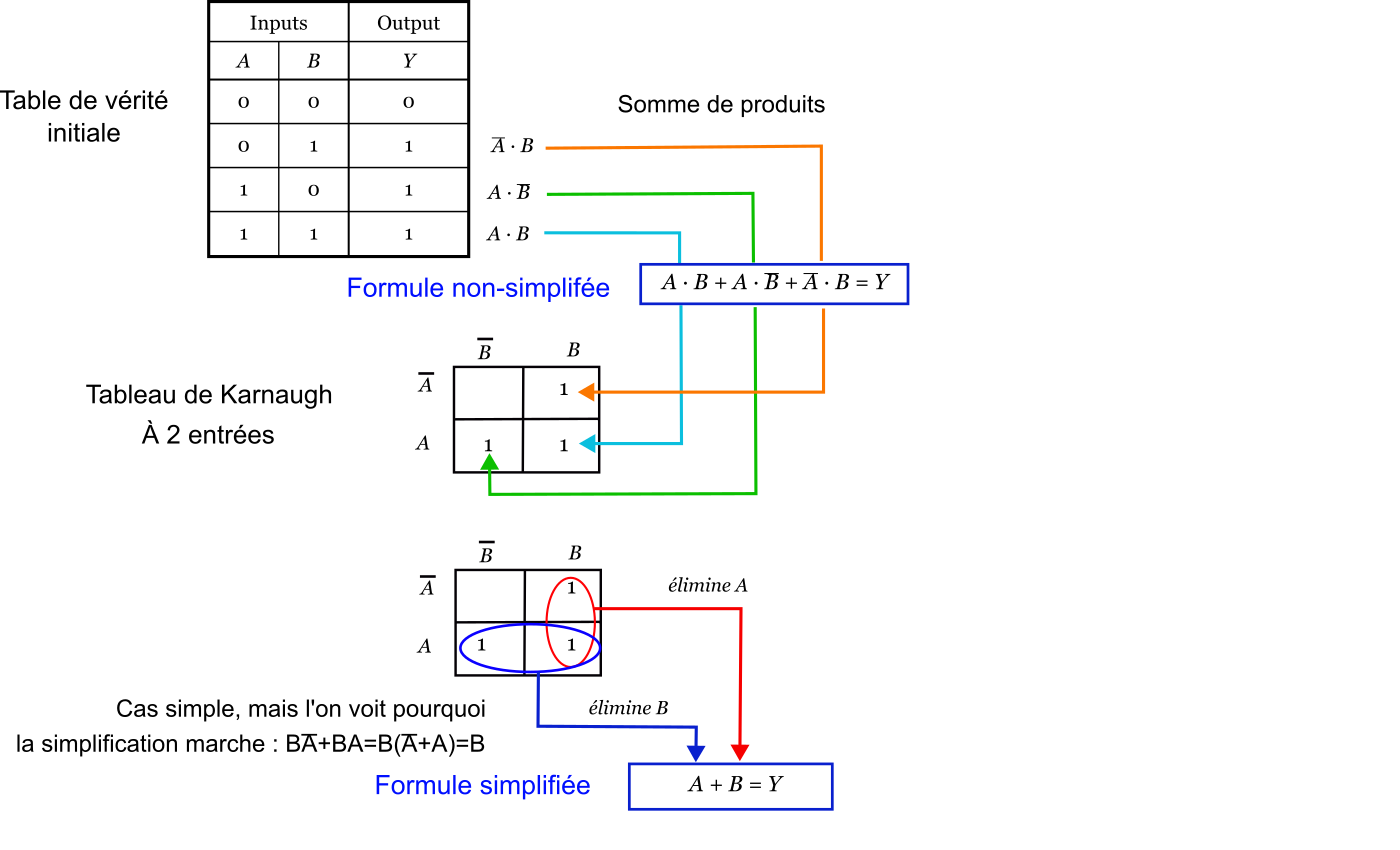
\includegraphics[scale=0.32]{./images/karnaugh_0.png}
      \end{center}
    \end{column}
  \end{columns}
\end{frame}

% --- Karnaugh : adjacence et principe ---
\begin{frame}{Tableau de Karnaugh : Adjacence et Principe}

    \begin{block}{Distance de Hamming}
        Pour deux vecteurs booléens \(u, v \in \mathbb{B}^n\), on définit :
        \[
            d_H(u,v) = \big|\{ i \in \{0,\dots,n-1\} : u_i \neq v_i \}\big|
        \]
        C'est le nombre de bits qui diffèrent entre \(u\) et \(v\).
    \end{block}

    \vspace{0.2cm}

    \begin{alertblock}{Définition — Adjacence}
        Deux cases du tableau de Karnaugh sont dites \textbf{adjacentes} si et seulement si : $d_H(u, v) = 1$
        % \[
        %     d_H(u, v) = 1
        % \]
        c'est-à-dire qu'elles ne diffèrent que par \textbf{une seule variable}.
    \end{alertblock}

    \vspace{0.1cm}

    \begin{columns}[T]
        \begin{column}{0.5\textwidth}
            \textbf{Justification :} si deux cases adjacentes ne diffèrent que par \(x\), leurs mintermes sont \(x \cdot m\) et \(\bar{x} \cdot m\), et :
            \[
                x \cdot m + \bar{x} \cdot m = (x + \bar{x}) \cdot m = m
            \]
            La variable \(x\) \textbf{disparaît}.
        \end{column}
        \begin{column}{0.45\textwidth}
            \textbf{Conséquence topologique :}\\
            Le tableau est \textbf{torique} — les bords opposés sont adjacents.

            \vspace{0.2cm}
            \textit{Exemple : \(000\) et \(100\) sont adjacents (\(d_H = 1\)).}
        \end{column}
    \end{columns}

\end{frame}

% --- Karnaugh : construction + code de Gray ---
\begin{frame}{Tableau de Karnaugh : Construction et Code de Gray}

    \begin{block}{Problème}
        Sur un tableau ordonné en binaire naturel, les cases voisines ne sont pas nécessairement adjacentes au sens de Hamming.
    \end{block}

    \vspace{0.3cm}

    \begin{columns}[T]
        \begin{column}{0.5\textwidth}
            \begin{alertblock}{Solution : Code de Gray}
                Ordonner les lignes et colonnes selon la suite :
                \[
                    00 \to 01 \to 11 \to 10
                \]
                Deux entrées consécutives diffèrent d'\textbf{un seul bit} (\(d_H = 1\)).
            \end{alertblock}
        \end{column}
        \begin{column}{0.45\textwidth}
            \centering
            \renewcommand{\arraystretch}{1.4}
            \begin{tabular}{|c|c|c|c|c|}
                \hline
                \(a \backslash bc\) & \(00\) & \(01\) & \textbf{\(11\)} & \(10\) \\
                \hline
                \(0\) & ~ & ~ & ~ & ~ \\
                \hline
                \(1\) & ~ & ~ & ~ & ~ \\
                \hline
            \end{tabular}
            % \begin{tabular}{|c|c|c|}
            %     \hline
            %     \(x \backslash y\) & \(0\) & \(1\) \\
            %     \hline
            %     \(0\) & \(\bar{x}\bar{y}\) & \(\bar{x}y\) \\
            %     \hline
            %     \(1\) & \(x\bar{y}\) & \(xy\) \\
            %     \hline
            % \end{tabular}

            \vspace{0.3cm}
            \textit{Chaque case = un minterme.}
        \end{column}
    \end{columns}

    \vspace{0.3cm}

    \textbf{Vérification :} \(00\) et \(01\) sont adjacents, \(01\) et \(11\) aussi, et ainsi de suite. La suite Gray garantit que toutes les cases voisines du tableau sont adjacentes au sens de Hamming.

\end{frame}

% --- Karnaugh : exemple 3 variables ---
\begin{frame}{Exemple : Tableau de Karnaugh à 3 Variables}

    \textbf{Fonction :} \(f(a,b,c) = \sum m(1,3,5,7)\)

    \vspace{0.3cm}

    \begin{columns}[T]
        \begin{column}{0.5\textwidth}
            \centering
            \renewcommand{\arraystretch}{1.6}
            \begin{tabular}{|c|c|c|c|c|}
                \hline
                \(a \backslash bc\) & \(00\) & \(01\) & \(11\) & \(10\) \\
                \hline
                \(0\) & 0 & \textbf{1} & \textbf{1} & 0 \\
                \hline
                \(1\) & 0 & \textbf{1} & \textbf{1} & 0 \\
                \hline
            \end{tabular}

            \vspace{0.3cm}

            \textit{Colonnes en code Gray : \(00, 01, 11, 10\).}
        \end{column}
        \begin{column}{0.48\textwidth}
            \textbf{Résolution :}

            \vspace{0.3cm}

            \begin{itemize}
                \item On regroupe les 4 \textbf{1} en un bloc \(2 \times 2\).
                \item Variables qui \textbf{changent} : \(a\) et \(b\).
                \item Variable qui \textbf{reste} : \(c = 1\).
                \item {\color{red} (Erreur dans le slideware distribué).} 
            \end{itemize}

            \vspace{0.4cm}

            \begin{exampleblock}{Résultat}
                \[
                    f = c
                \]
                De 4 mintermes à un seul littéral.
            \end{exampleblock}
        \end{column}
    \end{columns}


\end{frame}

% --- Karnaugh : regroupements formels ---
\begin{frame}{Regroupements : Règles Formelles}

    \begin{block}{Regroupement valide}
        Un regroupement est un sous-ensemble \(S\) de cases contenant des 1, tel que :
        \begin{itemize}
            \item \(|S| = 2^k\) pour un certain \(k \in \mathbb{N}\) ;
            \item \(S\) forme un \textbf{sous-cube} : produit cartésien de \(k\) paires d'entrées adjacentes.
        \end{itemize}
    \end{block}

    \vspace{0.3cm}

    \begin{alertblock}{Interprétation}
        Un sous-cube de taille \(2^k\) correspond à l'élimination de \(k\) variables par adjacence successive.
    \end{alertblock}

    \vspace{0.3cm}

    \begin{columns}[T]
        \begin{column}{0.5\textwidth}
            \textbf{Démarche :}
            \begin{enumerate}
                \item Remplir le tableau depuis la table de vérité.
                \item Identifier les \textbf{plus grands sous-cubes}.
                \item Vérifier que tous les 1 sont couverts.
                \item Lire le terme associé à chaque sous-cube.
            \end{enumerate}
        \end{column}
        \begin{column}{0.45\textwidth}
            \begin{exampleblock}{Limites}
                \begin{itemize}
                    \item Pratique jusqu'à 4 variables.
                    \item Difficile dès 5.
                    \item Au-delà : \textbf{Quine-McCluskey} ou \textbf{BDD}.
                \end{itemize}
            \end{exampleblock}
        \end{column}
    \end{columns}
\end{frame}


%========================================================================================
%\section{Logique Séquentielle}
%========================================================================================

%========================================================================================
%\section{Micro-architectures FSMD}
%========================================================================================

%========================================================================================
%\section{Introduction aux langages de description matériels : VHDL}
%========================================================================================

%========================================================================================

\end{document}
